\documentclass{article}
\usepackage{arxiv}

\captionsetup[figure]{labelfont=it,textfont={it}}


\title{A conditional permutation-based approach to test confounder and center effects in machine learning models}



\author{
  Tamas~Spisak \\
  Institute for Diagnostic and Interventional Radiology and Neuroradiology \\
  University Hospital Essen\\
  Hufelandstrasse 55, 45147 Essen \\
  \texttt{tamas.spisak@uk-essen.de} \\
  %% examples of more authors
  %% \AND
  %% Coauthor \\
  %% Affiliation \\
  %% Address \\
  %% \texttt{email} \\
  %% \And
  %% Coauthor \\
  %% Affiliation \\
  %% Address \\
  %% \texttt{email} \\
  %% \And
  %% Coauthor \\
  %% Affiliation \\
  %% Address \\
  %% \texttt{email} \\
}

\begin{document}
\maketitle

\begin{abstract} % 150 words
The lack of rigorous non-parametric statistical tests of confounder effects significantly hampers the development of robust, valid and generalizable predictive models in many fields of research.
Here I propose the \emph{partial} and \emph{full confounder tests}, that build on a recently established theoretical framework for permutation-based conditional independence testing and probe the null hypotheses of \emph{unconfounded} and \emph{fully confounded model}, respectively.
The proposed methods provide a strict control for Type-I errors and high statistical power, even in the presence of typical non-linear and non-normal dependencies between the target variable and the model output.
Applying the proposed tests on models trained on functional brain connectivity data from the Human Connectome Project and the Autism Brain Imaging Data Exchange dataset reveals confoudner effects that were previously unreported and found to be hard to correct for with state-of-the-art confound mitigation approaches.
The package \emph{mlconfound}\footnote{\href{https://mlconfound.readthedocs.io}{https://mlconfound.readthedocs.io}} can aid the assessment and improvement of the generalizability and neurobiological validity of predictive models and, thereby, foster the development of clinically useful machine learning biomarkers.
\end{abstract}


% keywords can be removed
\keywords{machine learning, predictive modelling, confounder test, conditional independence, conditional permutation}

%%%%%%%%%%%%%%%%%%%%%%%%%%%%%%%%%%%%%%%%%%%%%%%%%%%%%%%%%%%%%%%%%%%%%%%%%%%
\section{Introduction}

Predictive modelling and supervised learning methods have recently become increasingly important in biomedical research and hold promise for delivering biomarkers that substantially impact clinical practice and public health \citep{kent2018personalized}. When evaluating the usefulness and applicability of such markers, predictive performance (i.e. prognostic/diagnostic value) is far from being the only important consideration. Biomedical validity (i.e. whether the model is driven by biomedically relevant signal) and generalizability across contexts and populations are also crucial requirements for candidate biomarkers \citep{woo2017building}.

Spurious, out-of-interest associations between the predictor variables (features) and the prediction target - induced by so-called confounder effects - can be detrimental to the model's biomedical validity and generalizability. Many types of confounder effects can be distinguished.

First, measurement artifacts can obviously be considered as confounders. For instance, in-scanner head motion artifacts in magnetic resonance imaging (MRI)-based predictive models can be especially problematic, if the prediction target is also associated with motor function, like previously demonstrated, among others, in case of Alzheimer's disease \citep{rao2017predictive} attention deficit hyperactivity disorder (ADHD) \citep{couvy2016head, eloyan2012automated} or Autism Spectrum Disorder (ASD) \citep{spisak2014voxel, spisak2019optimal, gotts2013perils}. Likewise, eye-blink artifacts can result in confounder-bias in EEG-based markers of ASD  \citep{eldridge2014robust}.

Second, depending on the research question, demographic and psychometric variables can also be considered as confounders during predictive modelling. For instance, resting-state functional connectivity has been shown to be strongly predictive to age \citep{wang2012decoding, dukart2011age} and moderately to fluid intelligence \citep{he2020deep, cole2012global}. As fluid intelligence is known to decline with aging \citep{kievit2018neural}, models trained to predict intelligence can provide reasonable performance by picking up on solely age-related variance \citep{lohmann2021predicting, dubois2018distributed}. 

Third, batch effects or, in multi-center studies, center-effects can also cause significant bias in predictive models \citep{leek2010tackling, da2020performance} as the models can utilize such effects to explain (random or true) center/batch-differences in the predictive target. Such models will display worse-than-expected performance when applied on data from new centers/batches.

Various data cleansing, correction and harmonization approaches have been proposed to mitigate detrimental effects of confounders, ranging from sample matching \citep{rao2017predictive} and regression-based techniques \citep{rao2017predictive, dukart2011age, spisak2014voxel, abdulkadir2014reduction} to the popular non-parametric empirical Bayes-based method of \cite{johnson2007adjusting} and sophisticated deep-learning oriented solutions \citep{zhao2020training, hognon2019standardization}. However, it is often unclear which variables should be considered as confounders during harmonization and such approaches hold risks of eliminating signal-of-interest \citep{wachinger2021detect}.

Powerful and robust statistical tests to quantify the confounding effect of certain variables in predictive models could substantially foster both the the identification of confounders to correct for and the assessment of the effectiveness of various confound-mitigation and data harmonization approaches. Such methods, however, have to tackle the fact that the conditional distribution of the models' output, given the target, is often non-normal and non-linear, as a consequence of e.g. model regularization \citep{garcia2009study, kristensen2017whole}.

Recently, three dedicated techniques \citep{chaibub2019permutation, ferrari2020measuring, wachinger2021detect} have been proposed for quantifying confounder bias in predictive modelling.

The permutation-based approach of \cite{chaibub2019permutation} evaluates the null-hypothesis of no confounder bias via "restricted permutations" that retain the observed ratios of class labels within batches (often referred to as balanced permutations in the literature) However, as shown by \cite{southworth2009properties} and further discussed by \cite{hemerik2018exact}, balanced permutations do not provide a correct null behavior and can be invalid in certain circumstances. Indeed, \cite{ferrari2020measuring} demonstrated that this method does not guarantee a proper type I error control with biased classification problems.
The 'confounder index' (CI) proposed by \cite{ferrari2020measuring}, by design, does not provide any quantification of statistical significance.
Moreover, both approaches involve repeated re-fitting of the machine learning model, which might not be feasible for models with high computational complexity (especially when hyperparameters are optimized in a nested cross-validation).
The Kolmogorov Complexity-based causal inference test, as proposed by \cite{wachinger2021detect}, aims at determining whether it is more likely that the predictors are a direct cause of the target variable or, alternatively, there exists an unobserved random variable that is the cause of both. It's computation assumes 'faithfulness' (if two variables are independent, there is no direct influence between the two in the underlying graph) a strong condition that might not be fulfilled in many real applications (e.g. functional MRI is an \emph{indirect} measure of neural activation, rendering the alternative hypothesis of this test true in absence of any real confounder).

% todo: RO and CI: classification, KC: regression

In this paper, I formulate the 'confounder problem' as a special case of conditional independence testing \citep{dawid1979conditional}. This allows relating the problem to the seminal work of \cite{shah2020hardness}, who showed that, without placing some assumptions on the joint distribution of the involved variables, establishing a conditional independence test with a valid type I error control and non-trivial power is effectively impossible ("no free lunch" theorem).

Next, I utilize the permutation-based conditional independence framework of \cite{berrett2020conditional}, to construct two novel tests for evaluating the confounder-bias in predictive models.
The \emph{full confounder test} probes whether the model's predictive performance can be attributed exclusively to the confounder.
The \emph{partial confounder test} investigates whether the model utilizes any confounder-variance, when controlled for the target variable.
Both tests require only the target variable, the model predictions and the putative confounder as input, thus, they can be performed with a negligible extra computational cost (re-fitting the model is not required).
The tests set no assumption about the distribution of the model predictions.
The robustness of the type I error control and the statistical power of both tests are evaluated with simulated data (assuming non-normality).
The proposed tests are then applied on functional brain connectivity data to provide evidence of motion- and center-bias in a model trained on the Autism Brain Imaging Data Exchange (ABIDE) dataset \citep{di2014autism} and to evaluate the age and acquisition-batch dependence of fluid intelligence predictions on data from the Human Connectome Project.

%%%%%%%%%%%%%%%%%%%%%%%%%%%%%%%%%%%%%%%%%%%%%%%%%%%%%%%%%%%%%%%%%%%%%%%%%%%
\section{Methods}

\subsection{Notation and Background}

In a predictive modelling setting, let $\y$ denote the target variable, $\yhat$ denote model output, i.e. the predictions for $\y$ and let $\c$ denote a variable which is considered as a confounder (see Fig. \ref{fig:schematic}B). Let us assume, furthermore, that $\y$, $\yhat$ and $\c$ consist of independent and identically distributed (IID) data points $(y_i, \hat{y}_i, c_i) \in Y \times \\hat{Y} \times C$ for $i=1, \dots , n$ so that $\y=(y_1, \dots ,y_n)$, $\yhat=(\hat{y}_1, \dots, \hat{y}_n)$ and $\c=(c_1, \dots, c_n)$. 

Depending on the research question, the direct influence of $\c$ on the model predictions $\yhat$ is subject to be kept at a negligible level or it is to be proven that, at least, the model is not completely driven by $\c$.

Obviously, a strong association between $\yhat$ and $\c$ might indicate that the model is biased; it's predictions are driven by the confounder rather than information about the target variable.
Testing unconditional independence ($\yhat \independent \c$) between $\yhat$ and $\c$ (or any of the $\y$, $\yhat$, $\c$ variables) is, however, insufficient for the proper characterization of confounder-bias in predictive modelling.
For instance, even if $\yhat \independent \c$ is false, $\yhat$ might be only marginally dependent on $\c$, due to the dependence of both on $\y$. In other words, if the target variable $\y$ is significantly associated to the confounder variable $\c$, a model that is completely blind to $\c$ (and, therefore, unbiased) might still provide outputs $\yhat$ that are significantly associated with $\c$.

\subsubsection*{Conditional independence for testing confounder bias}

Instead of focusing on the unconditional independence between the confounder and the predictions, we shall consider the \emph{conditionally independence} between $\yhat$ and $\c$ given $\y$ (written as $\yhat \independent \c | \y$) which, by definition  \citep{dawid1979conditional}, means that $\mathbb{P}(\yhat, \c|\y) = \mathbb{P}(\yhat|\y)\mathbb{P}(\c|\y)$. The statistical test with this null hypothesis will be referred to as the \emph{partial confounder test}.

Alternatively, one might be also interested in testing $\yhat \independent \y | \c$. We will refer to the corresponding test as the \emph{full confounder test}.

 Conditional independence - in its general form - lies at the heart of several fundamental concepts in statistics and  plays an increasingly important role in various fields of applied statistics, particularly in biomedical applications \citep{spirtes2000causation, peters2016causal, fiedler2011mediation, candes2016panning}. Recently, \cite{shah2020hardness} have raised important concerns regarding conditional independence testing.
 Their "no free lunch" theorem implies that, without placing some assumptions on the joint distribution of $(\y, \yhat, \c)$, conditional independence testing is effectively impossible. In other words, neither the full nor the partial confounder tests can be constructed so that - for all distributions - they provides a valid type I error control and, at the same time, a non-trivial statistical power.

This result is in strong contrast to unconditional independence testing - where permutation tests  \citep{pitman1937significance, fisher1942189}, provide a general, distribution-free solution - and it has important implications for confounder testing in predictive modelling where the distribution of the model outputs, depending on the applied machine learning model, is unknown and often heavily non-normal.

Even if constructing fully non-parametric confounder tests was proven to be impossible, as demonstrated by \citep{candes2016panning} and \cite{berrett2020conditional}, valid and powerful conditional independence tests can be constructed with inputting distributional information about only two (out of the three) variables.
Specifically, the conditional permutation test (CPT) of Berret and colleagues samples from a non-uniform distribution over the set of possible permutations $\pi$ of one of the variables, based on its conditional distribution of the other variable. Thereby, it incorporates the information available on the conditional distribution of interest into the permutation-based inference in a statistically valid manner.

% fig:schematic
\begin{figure}
  \centering
  \resizebox{0.75\columnwidth}{!}{%
\tikzset{every picture/.style={line width=0.75pt}} %set default line width to 0.75pt        


\tikzset{every picture/.style={line width=0.75pt}} %set default line width to 0.75pt        

\begin{tikzpicture}[x=0.75pt,y=0.75pt,yscale=-1,xscale=1]
%uncomment if require: \path (0,300); %set diagram left start at 0, and has height of 300

%Shape: Circle [id:dp12907748114570317] 
\draw   (299.5,107) .. controls (299.5,93.19) and (310.69,82) .. (324.5,82) .. controls (338.31,82) and (349.5,93.19) .. (349.5,107) .. controls (349.5,120.81) and (338.31,132) .. (324.5,132) .. controls (310.69,132) and (299.5,120.81) .. (299.5,107) -- cycle ;
%Shape: Circle [id:dp12318976880062338] 
\draw   (397,39) .. controls (397,25.19) and (408.19,14) .. (422,14) .. controls (435.81,14) and (447,25.19) .. (447,39) .. controls (447,52.81) and (435.81,64) .. (422,64) .. controls (408.19,64) and (397,52.81) .. (397,39) -- cycle ;
%Shape: Circle [id:dp2655574667622329] 
\draw   (202,39) .. controls (202,25.19) and (213.19,14) .. (227,14) .. controls (240.81,14) and (252,25.19) .. (252,39) .. controls (252,52.81) and (240.81,64) .. (227,64) .. controls (213.19,64) and (202,52.81) .. (202,39) -- cycle ;
%Curve Lines [id:da9340239406716428] 
\draw    (250,28) .. controls (292,20) and (364,22) .. (400,28) ;
%Curve Lines [id:da6958426380393512] 
\draw    (239,61) .. controls (249,76) and (276,99) .. (299.5,107) ;
%Curve Lines [id:da8565840155201192] 
\draw    (349.5,107) .. controls (365,101) and (403,71) .. (410,60) ;

%Shape: Circle [id:dp9753164043561875] 
\draw   (475.5,257) .. controls (475.5,243.19) and (486.69,232) .. (500.5,232) .. controls (514.31,232) and (525.5,243.19) .. (525.5,257) .. controls (525.5,270.81) and (514.31,282) .. (500.5,282) .. controls (486.69,282) and (475.5,270.81) .. (475.5,257) -- cycle ;
%Shape: Circle [id:dp6395662810469516] 
\draw   (573,189) .. controls (573,175.19) and (584.19,164) .. (598,164) .. controls (611.81,164) and (623,175.19) .. (623,189) .. controls (623,202.81) and (611.81,214) .. (598,214) .. controls (584.19,214) and (573,202.81) .. (573,189) -- cycle ;
%Shape: Circle [id:dp786541411329625] 
\draw   (378,189) .. controls (378,175.19) and (389.19,164) .. (403,164) .. controls (416.81,164) and (428,175.19) .. (428,189) .. controls (428,202.81) and (416.81,214) .. (403,214) .. controls (389.19,214) and (378,202.81) .. (378,189) -- cycle ;
%Curve Lines [id:da22693900064180195] 
\draw    (426,178) .. controls (468,170) and (540,172) .. (576,178) ;
%Curve Lines [id:da6720989194231959] 
\draw    (415,211) .. controls (425,226) and (452,249) .. (475.5,257) ;
%Curve Lines [id:da8140666812849395] 
\draw    (525.5,257) .. controls (541,251) and (579,221) .. (586,210) ;
%Shape: Circle [id:dp471386481785639] 
\draw   (50,256) .. controls (50,242.19) and (61.19,231) .. (75,231) .. controls (88.81,231) and (100,242.19) .. (100,256) .. controls (100,269.81) and (88.81,281) .. (75,281) .. controls (61.19,281) and (50,269.81) .. (50,256) -- cycle ;
%Shape: Rectangle [id:dp8617145222488287] 
\draw   (156,237) -- (240,237) -- (240,277) -- (156,277) -- cycle ;
%Shape: Circle [id:dp8776576784951928] 
\draw   (290,256) .. controls (290,242.19) and (301.19,231) .. (315,231) .. controls (328.81,231) and (340,242.19) .. (340,256) .. controls (340,269.81) and (328.81,281) .. (315,281) .. controls (301.19,281) and (290,269.81) .. (290,256) -- cycle ;
%Shape: Circle [id:dp2868603849402189] 
\draw   (174,190) .. controls (174,176.19) and (185.19,165) .. (199,165) .. controls (212.81,165) and (224,176.19) .. (224,190) .. controls (224,203.81) and (212.81,215) .. (199,215) .. controls (185.19,215) and (174,203.81) .. (174,190) -- cycle ;
%Callout Right Arrow [id:dp26184503306970397] 
\draw   (46.55,225.27) -- (106,225.27) -- (106,250) -- (133,250) -- (133,241) -- (155.55,255.27) -- (133,269.55) -- (133,260.55) -- (106,260.55) -- (106,285.27) -- (46.55,285.27) -- cycle ;
%Right Arrow [id:dp7986276189609152] 
\draw   (240,250) -- (268,250) -- (268,241) -- (290,255.5) -- (268,270) -- (268,261) -- (240,261) -- cycle ;
%Shape: Circle [id:dp9535423837564185] 
\draw   (50,190) .. controls (50,176.19) and (61.19,165) .. (75,165) .. controls (88.81,165) and (100,176.19) .. (100,190) .. controls (100,203.81) and (88.81,215) .. (75,215) .. controls (61.19,215) and (50,203.81) .. (50,190) -- cycle ;
%Straight Lines [id:da6172567079022628] 
\draw    (75,215) -- (75,231) ;
%Straight Lines [id:da8731068989736062] 
\draw    (198,238) -- (198,215) ;

% Text Node
\draw (165,251) node [anchor=north west][inner sep=0.75pt]   [align=left] {ML model};
% Text Node
\draw (9,6) node [anchor=north west][inner sep=0.75pt]   [align=left] {\textbf{A}};
% Text Node
\draw (9,146) node [anchor=north west][inner sep=0.75pt]   [align=left] {\textbf{B}};
% Text Node
\draw (494,252.4) node [anchor=north west][inner sep=0.75pt]    {$\c$};
% Text Node
\draw (591.5,180.4) node [anchor=north west][inner sep=0.75pt]    {$\yhat$};
% Text Node
\draw (396,184.4) node [anchor=north west][inner sep=0.75pt]    {$\y$};
% Text Node
\draw (484,198) node [anchor=north west][inner sep=0.75pt]   [align=left] {CPT};
% Text Node
\draw (67,251.4) node [anchor=north west][inner sep=0.75pt]    {$X$};
% Text Node
\draw (308.5,247.4) node [anchor=north west][inner sep=0.75pt]    {$\yhat$};
% Text Node
\draw (191,185.4) node [anchor=north west][inner sep=0.75pt]    {$\y$};
% Text Node
\draw (318,102.4) node [anchor=north west][inner sep=0.75pt]    {$Z$};
% Text Node
\draw (415.5,34.4) node [anchor=north west][inner sep=0.75pt]    {$Y$};
% Text Node
\draw (219,34.4) node [anchor=north west][inner sep=0.75pt]    {$X$};
% Text Node
\draw (308,48) node [anchor=north west][inner sep=0.75pt]   [align=left] {CPT};
% Text Node
\draw (68,185.4) node [anchor=north west][inner sep=0.75pt]    {$\c$};


\end{tikzpicture}

    }
  \caption{Schematic diagram of using CPT in a predictive modelling context. \\ \textbf{(A)} CPT was originally proposed to be used on the feature variable $X$, target variable $Y$ and confounders $Z$. \textbf{(B)} The proposed use of CPT in predictive modelling requires the model to be fitted first, to obtain the model's prediction $\yhat$ on $\y$. CPT is then utilized on the triplet $(\y, \yhat, \c)$, to test hypotheses $\yhat \independent \c | \y$ or $\y \independent \yhat | \c$.}
  \label{fig:schematic}
\end{figure}


As many related papers, the work of \cite{berrett2020conditional} was formalized as a (semi-)supervised learning approach, where $X$ is a set of predictors (features), $Y$ is the target variable and $Z$ is a potential confounder. In this setting, testing the null hypothesis $X \independent Y | Z$ aims to determine, whether the features $X$ still affect $Y$, when controlling for $Z$.
For instance, in genome-wide association studies, CPT can be used to determine whether a particular genetic variant $X$ affects a response $Y$ such as disease status or some other phenotype, even after controlling for the rest of the genome, encoded in $Z$.

In this paper, a different setting is considered, where the supervised learning model is already fitted and we are focusing on model diagnostics, by testing the triplet $(\y,\yhat, \c)$. The conceptual difference between the original and the proposed application of CPT is depicted on Fig. \ref{fig:schematic}.

Within this setting, conditional independence testing and, specifically, the framework of conditional permutation testing allows investigating three different null hypotheses corresponding to the $(\y, \yhat, \c)$ triplet. As listed in Table \ref{tab:conditional-independence-cases}, testing the null hypothesis $\y \independent \yhat | \c$ (option 1, full confounder testing) investigates whether the model predictions are likely explainable solely with the confounder, i.e. whether the model is exclusively confounder-driven. Testing $\y \independent \c | \yhat$ (option 2) addresses the question whether the model captures all the variance in $c$ when predicting $y$. Testing the null hypothesis $\yhat \independent \c | \y$ (option 3, partial confounder testing) examines, whether the dependence of the model output on the confounder can likely be explained by the confounder's dependence on the target variable, i.e. whether there is any confounder bias in the model.

% tab:conditional-independence-cases
\renewcommand{\arraystretch}{1.2}
\begin{table}[]
\centering
\begin{tabular}{l|rp{60mm}|c|>{\centering\arraybackslash}m{30mm}}
 &  & H0  & assumption needed for: & no assumptions about the distribution of: \\
\hline
\textbf{1.} & $\y \independent \yhat | \c$ \quad  & model exclusively driven by confounder (full confounder test) & $Q(\cdot|\c)$ & $\yhat$ or $\y$ \\
%\hline
\textbf{2.} & $\y \independent \c | \yhat$ \quad & model captures all variance in confounder (not of interest) & $Q(\cdot|\yhat)$ & $\y$ or $\c$ \\
%\hline
\textbf{3.} & $\yhat \independent \c | \y$  \quad &  model does not capture more confound than what is present in the target (partial test) & $Q(\cdot|\y)$ & $\yhat$ or $\c$ \\
\end{tabular}
\caption{\label{tab:conditional-independence-cases} Possibilities when testing conditional independence in potentially biased predictive models. \\The table lists the three possible null hypotheses (H0), and the variables where assumption about the joint/conditional distributions is required/not required.   ($y$: prediction target, $\yhat$: predictions, $\c$: confounder variable) }
\end{table}

Option 3, i.e. partial confounder testing is typically of interest when testing confounder bias of predictive models. Option 1, i.e. full confounder testing, might be also useful in diagnostics of predictive models, especially in the exploratory phase of model construction. Option 2 seems less appealing for model diagnostics and importantly, in this case the proposed variety of the CPT framework does not allow constructing a test which is non-parametric on $\yhat$.

Below, CPT is adapted for partial confounder testing (option 3). The formulation of the full confounder test (option 1) is analogous and given in Supplementary Material \ref{sup:full-test}.
\subsubsection*{The partial confounder test}

The partial confounder test generates a null-distribution for an arbitrary predefined test statistic $T(\y,\yhat,\c)$ by sampling permutation based "copies" of $\c$,

\begin{equation}
    c_i^{(j)} \sim Q(\cdot|y_i)
     \label{eq:cond-copy}
\end{equation}

where, $Q(.|y)$ denotes the conditional distribution of $\c$ given $\y=y$ and $j=1,\dots, m$ indexes the "copy" of $\c$ so that

$$ \c^{(j)} = (c_1^{(j)}, \dots, c_n^{(j)}) = (c_{\pi_1^{(j)}}, \dots, c_{\pi_n^{(j)}}) =  \c_{\boldsymbol{\pi}^{(j)}} $$

is a permutation of the original vector $\c = (c_1, \dots, c_n)$, with its elements reordered according to the permutation $\quad \boldsymbol{\pi} \in S_n$ where $S_n$ denote the set of all permutations on the indices $\{1,\dots,n\}$.

As shown in \citep{berrett2020conditional}, to ensure that Eq. \ref{eq:cond-copy} holds, the $\c_{\boldsymbol{\pi}^{(j)}}$ copies must be drawn so that:

\begin{equation}
    \label{eq-pperm}
    \mathbb{P}(\boldsymbol{ \pi }^{(j)} = \boldsymbol{ \pi } | \y,\yhat,\c) = \frac{q^n(\c_{\boldsymbol{ \pi }} | \y)}{\sum_{\boldsymbol{ \pi } ' \in S_n} q^n(\c_{\boldsymbol{ \pi } ' } | \y)}
\end{equation}


that is, according to the $q^n(\cdot|\y) := q(\cdot | y_1) \dots q(\cdot|y_n)$ product density corresponding to the conditional distribution $Q(\cdot|\y)$. Note that Eq. \ref{eq-pperm} does not necessarily assume a continuous distribution.

This mechanism creates copies $\c^{(1)}, \dots ,\c^{(m)}$ so that under the null hypothesis ($\yhat \independent \c | \y$), the triples 

$$(\y,\yhat,\c), (\y, \yhat, \c^{(1)}),\dots, (\y, \yhat, \c^{(m)})$$

are all identically distributed and so are the 

$$T(\y,\yhat,\c), T(\y, \yhat, \c^{(1)}),\dots,T(\y, \yhat, \c^{(m)})$$

test statistics, as well.

As long as the numerator of Eq. \ref{eq-pperm} is non-zero for all $c_\pi \in C$ and $y \in Y$, the conditional permutations constitute an algebraic group, thus, as shown by \citep{hemerik2018exact}, an unbiased estimate of the p-value under the null can be obtained as:
$$ p= \frac{\sum_{j=1}^m \mathbb{1} \{T(\y, \yhat, \c^{(j)}) \geq T(\y, \yhat, \c) \}  }{m}$$

While the group property of the conditioned permutations provides a straightforward proof for the validity of the approach, for an alternative verification see the proof of Theorem 1 in \citep{berrett2020conditional}.

While the required permutations could be theoretically sampled with a simple Metropolis-Hastings algorithm that draws uniformly from $S_n$ at random, this way the acceptance ratio would be extremely low, even for moderate $n$ (except there is very low dependence of $\c$ on $\y$), resulting in slow mixing times. The partial confounder test can be, however, efficiently implemented with the parallelized pairwise Markov-Chain Monte Carlo sampler of \cite{berrett2020conditional} (Algorithm 1), that draws disjoint pairs in parallel and decides whether or not to swap them randomly, according to the odds ratio calculated from the conditional densities belonging to the original and swapped data. The acceptance odds ratio of swapping indices $i$ and $j$ is:

\begin{equation}
\frac{ q(c_j | y_i) q(c_i | y_j)}{q(c_i | y_i) q(c_j | y_j) }
=
\ell(c_j | y_i) + \ell(c_i | y_j) - \ell(c_i | y_i) - \ell(c_j | y_j) 
\label{eq:accept-odds}
\end{equation}

where $\ell$ denotes the log-likelihood.

In their Theorem 2, \cite{berrett2020conditional} verify that the resulting Markov Chain yields the desired stationary distribution, even if the number of steps is small.

\subsubsection*{Gaussian conditional log-likelihood}


Obtaining a relatively accurate, independent estimate of $D(\cdot|\y)$ (of any shape) for CPT inference is important. Berrett and colleagues recommend to use a large independent sample to obtain the log-likelihood matrix that represents the conditional distribution $D(\cdot|Z)$. This approach might be often viable in semi-supervised learning settings where unlabelled data $(X, Z)$ are easier to obtain than labelled data $(X, Y, Z)$.
Since in the proposed predictive modelling setting, normality might be often a reasonable assumption for $\y$ and $\c$ (but not for $\yhat$), it is possible to fall back to Gaussian assumptions and thereby eliminate the need for a large, independent sample to estimate $D(\cdot|\y)$.

In case of continuous target, a linear regression model  can be fitted:

\begin{equation}
    \label{eq:linreg}
    \c = \alpha + \beta \y + \boldsymbol{e}
\end{equation}


with the assumption that the residual error follows a Gaussian distribution. If we write $\boldsymbol{\mu} = \alpha + \beta \y$ and $\sigma$ denotes the standard deviation of the residual $\boldsymbol{e}$, then the conditional distribution of interest can also be assumed to be normal with the parameters:

$$ (\c|\y=y_i) \sim \mathcal{N}\{\mu_i, \sigma^2\}$$

and the log-likelihood, that is to be used in Eq. \ref{eq:accept-odds}, can be computed simply as the log of the corresponding probability density function:

$$ \ell(c_i|y_j) = - \frac{1}{2} \Big(\frac{c_i-\mu_j}{\sigma}\Big)^2 - ln(2 \pi \sigma)   $$

In the case of categorical $c$, a multinomial logistic regression model can be used to obtain $D(\cdot|\y)$, with the extra assumption of non-complete separation if $y$ is also categorical (for an invertible Hessian, see e.g. \citep{bohning1992multinomial}).

Importantly, both the linear and the multinomial logistic regression approaches guarantee that the numerator of Eq. \ref{eq-pperm} is always greater than zero and the group property for the permutations holds.

Note that from the three options for conditional independence-based null hypotheses enumerated in Table \ref{tab:conditional-independence-cases}, for option 2, the proposed approach can not provide a test that is assumption-free about $yhat$, as the variable on which the independence is conditional must be always the predictor variable in Eq. \ref{eq:linreg}. However, as discussed above, this option is of low practical relevance, anyway.
Pleasingly,  the proposed Gaussian regression-based conditional likelihood estimation ensures that no assumptions on $\yhat$ have to be made for the practically relevant options 1 and 3, i.e. for the full and partial confounder tests.

In theory, any predefined test statistic $T$ can be used with the proposed approach. The python package \emph{mlconfound}, implementing the proposed full and partial confoudner tests, utilizes the coefficient of determination ($R^2$ or pseudo $R^2$ in case of categorical confounder or classification \citep{starkweather2011multinomial}) as a test statistic:

$$T(\y, \yhat, \c) = R^2(\yhat, \c)$$ 

and

$$T(\y, \yhat, \c^{(j)}) = R^2(\yhat, \c^{(j)})$$ 

which allows interpretable, two tailed inference about confoudner-bias in predictive modelling.

%%%%%%%%%%%%%%%%%%%%%%%%%%%%%%%%%%%%%%%%%%%%%%%%%%%%%%%%%%%%%%%%%%%%%%%%%%%
\begin{figure}[!b]
  \centering
  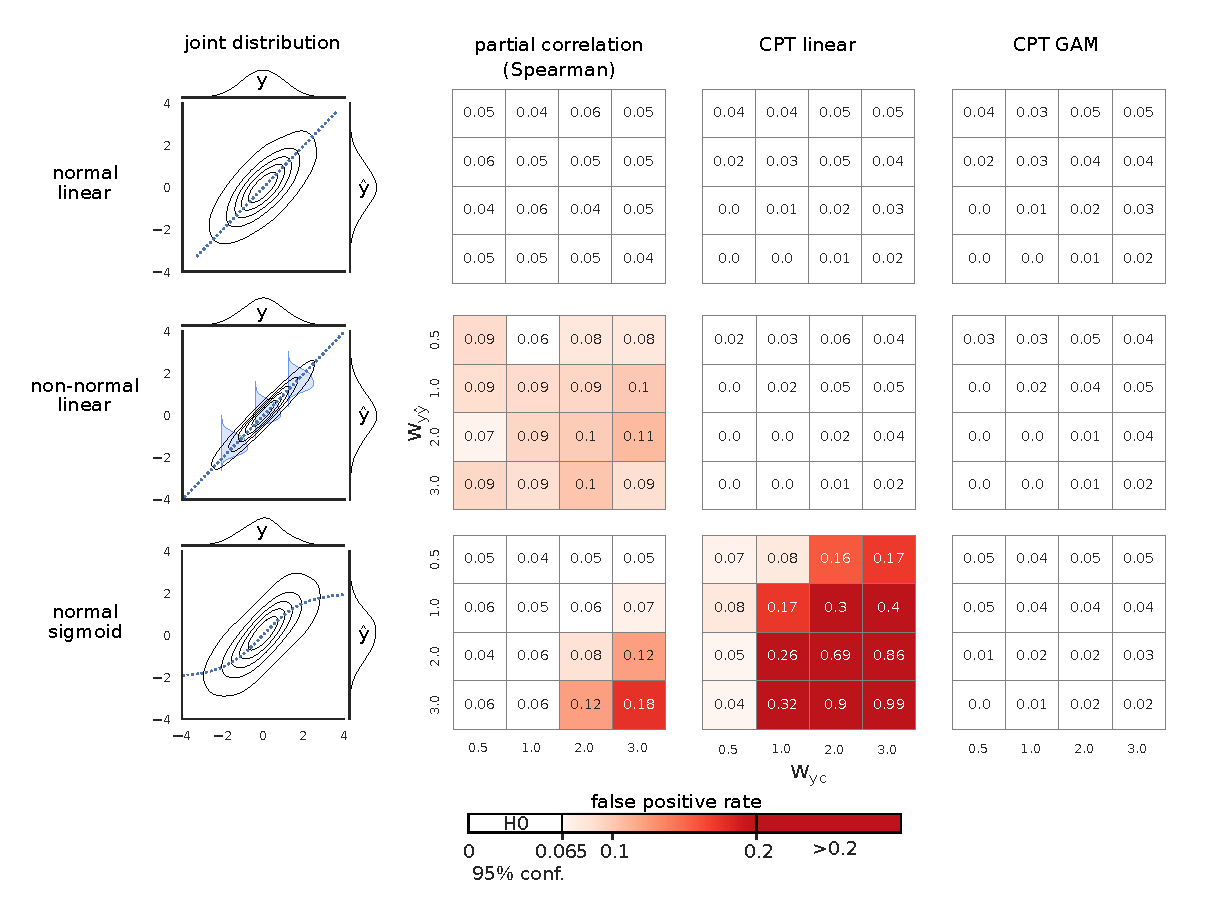
\includegraphics[width=0.75\paperwidth]{fig/sim_h0_demo.eps}
  \caption{\textbf{Type-I error control and power of the conditional permutation-based confound testing for predictive modelling in normally distributed simulated data}. \\
  Heatmaps depict positive rates (ratio of p-values lower than 0.05, color coded as shown by the palette at the bottom) in various simulations settings (100 simulations per tile) with different covariance between the target and the confounder (given as $R^2_{y,c}$ on the vertical axes of the heatmaps), for different sample sizes (N, horizontal axes).
  Rows and columns correspond to simulations with different signal-in-prediction (y+c) and confound-to-signal values, respectively. The first row and the first column contain simulations under H0 (no confounder bias) and separated form the simulations under the alternative hypothesis with dashed line. Positive rates for the simulations under the null and alternative hypotheses can be interpreted as type I error rate and statistical power, respectively. The higher confidence limit for the type I error rates is 0.11 for each tile, with 5 tiles expected to pass it form all H0 tiles.
  The actual weights $w_{Y}$, $w_{C}$ and $w_{e}$ are depicted at the bars on top of each heatmap and color coded as shown in the legend at the bottom. Above each heatmap, the strengths of the associations of $\hat{y}$ to $Y$ and $C$, respectively, are given with $R^2$ values averaged over all simulation cases of the heatmap.
  }
  \label{fig:sim-normal}
\end{figure}


\subsection{Validation on simulated data}

Using CPT to test confounder-bias in predictive modelling allows relaxing assumptions on $\yhat$ (for both the partial and the full test) but - in line with the "no free lunch" theorem, requires knowing - or putting assumptions on - the joint distribution of the other two variables ($\yhat$ and $\c$). 
\cite{berrett2020conditional} give a detailed analysis of the robustness of their CPT approach when estimating the conditional distribution with re-using the tested data and, also, against misspecifying the conditional distribution of interest.

While their findings are largely applicable to the proposed tests, here I extend those results by performing simulations in a form that is accessible for power calculations in predictive modelling (considering various weights of the confounder and the target signals in $\yhat$ and in the case of varying levels of covariance between $\y$ and $\c$).
Moreover, I perform a thorough investigation of the robustness of the test against the violation of normality (for both $(\y, \c)$ and $\yhat$).

Simulations are performed separately for the 'partial' and 'full' conditional confound tests.

\subsubsection*{Gaussian Simulations}
As  a first step, the target variable $\y$ and the confounder variable $\c$ are drawn randomly from a multivariate normal distribution:

$$ \y, \c \sim \mathcal{N}(\mu_0, \Sigma_\sigma) $$

where $\mu_0=(0, 0)$ and the covariance matrix is given as:
$\Sigma_\sigma = \big(\begin{smallmatrix}
  1 & \sigma\\
  \sigma & 1
\end{smallmatrix}\big)$ with $\sigma$ (i.e. the covariance between $\y$ and $\c$) being a free parameter of the simulation.

Next, the simulated predicted values are constructed:
 with an additive model:
$$ \yhat = w_y \y + w_c \c + w_e \boldsymbol{e}$$

so that $w_y + w_c + w_e = 1$, where $\boldsymbol{e} \sim \mathcal{N}(0,1)$ is the noise component.

To test the implementation for categorical variables, simulated $\y$, $\yhat$ and $\c$ variables are binarized by thresholding at 0.

For more straightforward interpretation and visualization of the simulation results, the 'confound-to-target' and the 'signal-in-prediction' parameters are defined as

$$ w_{c/y} = w_c / w_y $$

and

$$ w_{c+y} = w_c + w_y $$

respectively.

\subsubsection*{Introducing non-normality}

Non-normality is introduced by applying the \emph{sinh-arcsinh} transformation of \cite{jones2009sinh} on the simulated variables:

$$\boldsymbol{x}' = sinh(\delta sinh^{-1}(\boldsymbol{x}) - \epsilon)$$

where the parameters $\delta$ and $\epsilon$ control the kurtosis and skewness of the resulting \emph{sinh-arcsinh} distribution, with $\delta=1$ and $\epsilon=0$ producing the identity function (i.e. no non-normality introduced).

\subsubsection*{Simulation cases}

In the simulation procedure for the 'partial' confound test, 100 repetitions were performed of all combination of the following parameter values: 
\begin{itemize}
    \item covariance of $\c$ and $\y$: $\sigma \in \{0, 0.2, 0.4, 0.6, 0.8\}$
    \item confound-to-target: $w_{c/y} \in \{0, 0.1, 0.3, 0.5, 1\}$
    \item signal-in-prediction: $w_{c+y} \in \{0, 0.3, 0.6, 0.9\}$
    \item sample size: $n \in \{50, 100, 500, 1000\}$
\end{itemize}

For testing 'full' confounder bias, identical parameters were used, except that instead of the 'confound-to-target' parameter $ w_{c/y}$ we used the 'target-to-confound' parameter $ w_{y/c} = w_y/ w_c $, but with the same parameter values $w_{y/c} \in \{0, 0.1, 0.3, 0.5, 1\}$.

Next to the above described normally distributed simulation scenario, four analogous, but \emph{sinh-arcsinh} transformed scenarios were also investigated, with $\delta \in \{1, 1.05, 1.5, 5\}$ $\epsilon \in \{1, 3, 5, 10\}$ 

The 'partial' and 'full' confound tests, as implemented in version 0.9.0 of the package \emph{'mlconfound'} were run with default parameters, that is 1000 permutations and 50 Markov-chain Monte-Carlo steps to generate the conditioned permutations and by implying categorical variables, where needed.

Analysis code used for simulations is available\footnote{https://github.com/pni-lab/mlconfound/blob/master/validation/simulation.py} in the github repository of the 'mlconfound' package.

\subsection{Application on functional brain connectivity data}

The usefulness of the proposed confounder tests is demonstrated by applying them for predictive classification and regression models based on functional brain connectivity data, processed with different confound-mitigation approaches. 

'Partial' and 'full' confound testing was performed with default parameters (10000 permutations, 50 Markov-chain Monte Carlo steps) as implemented in version 0.9.0 of the package \emph{'mlconfound'}. Unconditional dependence across the involved variables was investigated with conventional permutation test on the $R^2$ values, with 1000 permutations. 

\subsubsection*{HCP: testing age- and acquisition batch-bias in fluid intelligence prediction}

Human Connectome Project contains imaging and behavioral data of approximately 1200 healthy subjects \citep{van2013wu}. Preprocessed resting state fMRI connectivity data (partial correlation matrices) \citep{glasser2013minimal} as published with the HCP1200 release (N=999 participants with functional connectivity data) were used to build models that predict individual fluid intelligence scores (IQ), measured with Penn Progressive Matrices \citep{duncan2000neural}.

To ensure normality, fluid intelligence scores were non-linearly transformed to normal distribution with the quantile transformation \citep{beasley2009rank} as implemented in \emph{scikit-learn} \citep{pedregosa2011scikit} (see Supplementary Figure \ref{fig:hcp-hist} for details).

Features (functional connectivities across 100 group-independent component analysis based regions) were either (i) considered in their raw form or were subject to confound mitigation approaches by (ii) feature regression \citep{rao2017predictive} or (iii) COMBAT \citep{johnson2007adjusting, fortin2018harmonization}.
The feature mitigation strategies were separately applied for acquisition batch and age group as confounder variable.

The total of 5 types of features (raw, regressing out acquisition batch, regressing out age group, COMBAT with acquisition batch, COMBAT with age group) were independently incorporated into a scikit-learn-based \citep{pedregosa2011scikit} machine learning procedure aiming to predict the individual fluid intelligence scores with a ridge-regression \citep{hoerl1970ridge}. The $\alpha$ parameter of the ridge model was considered as a hyperparameter ($\alpha \in \{0.00001, 0.0001, 0.001, 0.01, 0.1, 1, 10, 100, 1000, 10000, 100000\}$) and optimized in a nested cross-validation (cv) with 10 folds both in the inner and the outer cv-s and with mean squared error as optimization metric. Confound mitigation was performed inside of the outer cross-validation loop, to avoid leakage.

Analysis code is available as jupyter notebook\footnote{\href{https://github.com/pni-lab/mlconfound/tree/master/notebooks/analysis\_hcp.ipynb}{https://github.com/pni-lab/mlconfound/tree/master/notebooks/analysis\_hcp.ipynb}} in the github repository of the 'mlconfound' package.


\subsubsection*{ABIDE: testing motion- and center-bias in predictive models of autism spectrum disorder diagnosis}

The proposed tests were applied to provide evidence of center- and  motion-bias in diagnostic predictive models of autism spectrum disorder (ASD), trained on the Autism Brain Imaging Data Exchange (ABIDE) dataset \citep{di2014autism} involving 866 participants; ASD: 402, healthy control (HC): 464. Preprocessed regional timeseries data was obtained as shared with the paper \citep{dadi2019benchmarking} which was based on preprocessed image data provided by the Preprocessed Connectome Project \citep{craddock2013neuro}.

Tangent correlation across the timeseries of the n=122 regions of the BASC \citep{bellec2010multi} atlas) was computed with nilearn\footnote{\href{http://nilearn.github.io/}{http://nilearn.github.io/}} \citep{huntenburg2017loading, esteve2015big}. 

The resulting functional connectivity estimates were considered as features either (i) in their raw form or after applying (ii) feature regression \citep{rao2017predictive} or (iii) COMBAT \citep{johnson2007adjusting, fortin2018harmonization}.
The investigated confounder variables were 'imaging center' and in-scanner motion, as measured by the mean framewise displacement of \cite{power2014methods}).
Mean FD was non-linearly transformed to normal distribution with the quantile transformation \citep{beasley2009rank} as implemented in \emph{scikit-learn} \citep{pedregosa2011scikit} (see Supplementary Figure \ref{fig:abide-hist} for details).

As COMBAT is not able to handle continuous variables (since it was primarily designed to remove "batch-effects"), motion was binned into 10 groups, based on equdistant data quantiles ranging from 0 to 1.

The total of five types (raw, feature regression of site, feature regression of motion, COMBAT with site, COMBAT with motion) of features were independently incorporated into a scikit-learn-based \citep{pedregosa2011scikit} machine learning procedure aiming to predict the diagnosis (DX: ASD vs. HC) with a L2-regularized logistic regression (as e.g. in \citep{dadi2019benchmarking}). The $C$ parameter of the model was considered as a hyperparameter ($C \in \{0.1, 1, 10\}$) and optimized in a nested cross-validation (cv) with 10 folds both in the inner and the outer cv-s and with area under the receiver operator curve (AUC under ROC) as optimization metric. Confound mitigation was performed inside of the outer cross-validation loop, to avoid leakage.

Confounder testing was performed on the class probabilities (instead of the predicted labels).

Analysis code is available as jupyter notebook\footnote{\href{https://github.com/pni-lab/mlconfound/tree/master/notebooks/analysis\_abide.ipynb}{https://github.com/pni-lab/mlconfound/tree/master/notebooks/analysis\_abide.ipynb}} in the github repository of the 'mlconfound' package.

%%%%%%%%%%%%%%%%%%%%%%%%%%%%%%%%%%%%%%%%%%%%%%%%%%%%%%%%%%%%%%%%%%%%%%%%%%%
\section{Results}

\begin{figure}[!b]
  \centering
  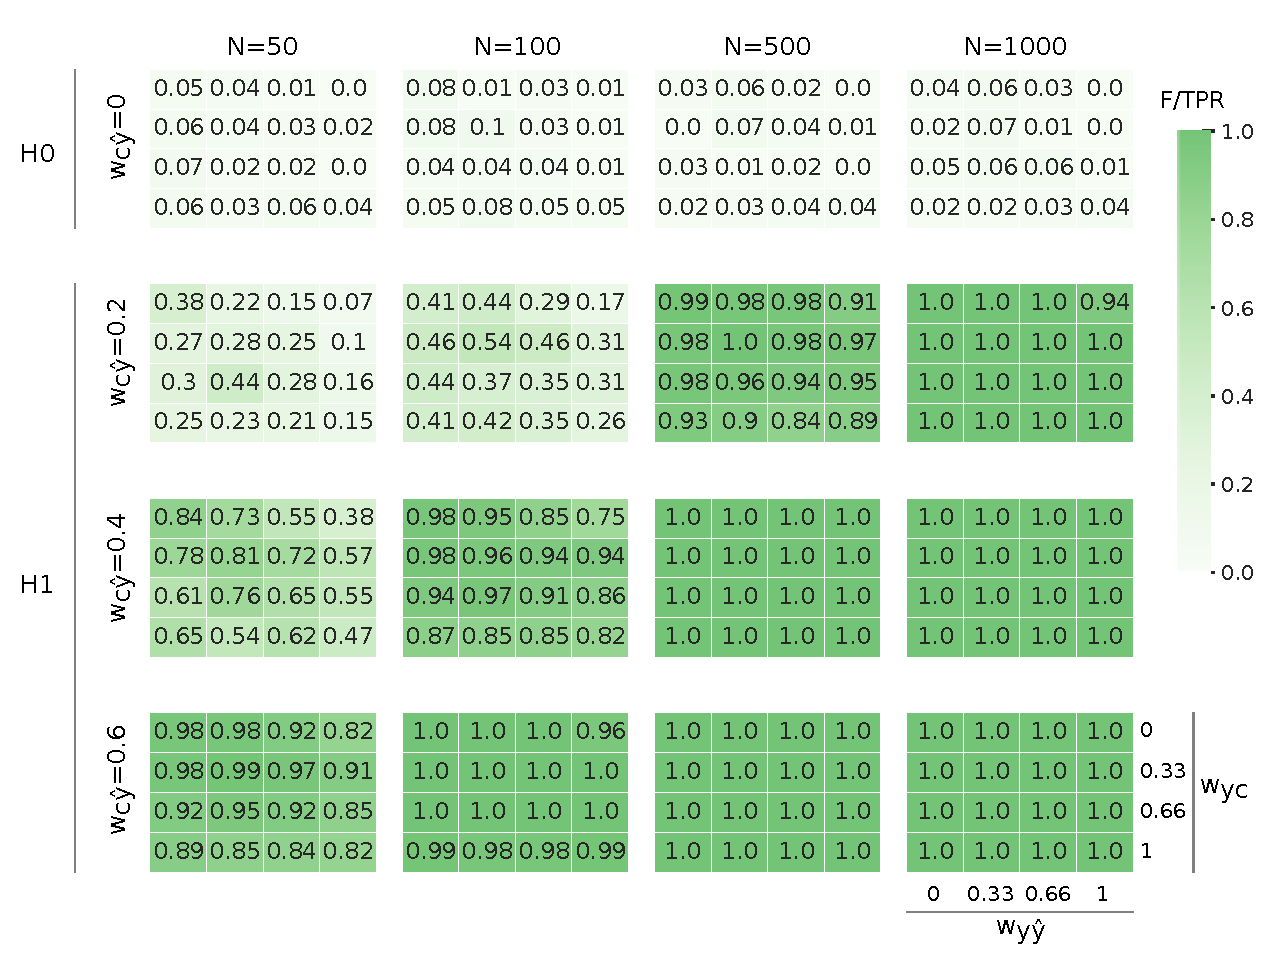
\includegraphics[width=0.75\paperwidth]{fig/sim_normal.eps}
  \caption{\textbf{Type-I error control and power of the conditional permutation-based confound testing for predictive modelling in normally distributed simulated data}. \\
  Heatmaps depict positive rates (ratio of p-values lower than 0.05, color coded as shown by the palette at the bottom) in various simulations settings (100 simulations per tile) with different covariance between the target and the confounder (given as $R^2_{y,c}$ on the vertical axes of the heatmaps), for different sample sizes (N, horizontal axes).
  Rows and columns correspond to simulations with different signal-in-prediction (y+c) and confound-to-signal values, respectively. The first row and the first column contain simulations under H0 (no confounder bias) and separated form the simulations under the alternative hypothesis with dashed line. Positive rates for the simulations under the null and alternative hypotheses can be interpreted as type I error rate and statistical power, respectively. The higher confidence limit for the type I error rates is 0.11 for each tile, with 5 tiles expected to pass it form all H0 tiles.
  The actual weights $w_{Y}$, $w_{C}$ and $w_{e}$ are depicted at the bars on top of each heatmap and color coded as shown in the legend at the bottom. Above each heatmap, the strengths of the associations of $\hat{y}$ to $Y$ and $C$, respectively, are given with $R^2$ values averaged over all simulation cases of the heatmap.
  }
  \label{fig:sim-normal}
\end{figure}

The conditional permutation based 'partial' and 'full' confound tests for predictive modelling have been implemented in the python package \emph{mlconfound}\footnote{\href{https://mlconfound.readthedocs.io}{https://mlconfound.readthedocs.io}}.

\subsection{Simulations}

\subsubsection*{Type I error}

\begin{figure}[!b]
  \centering

  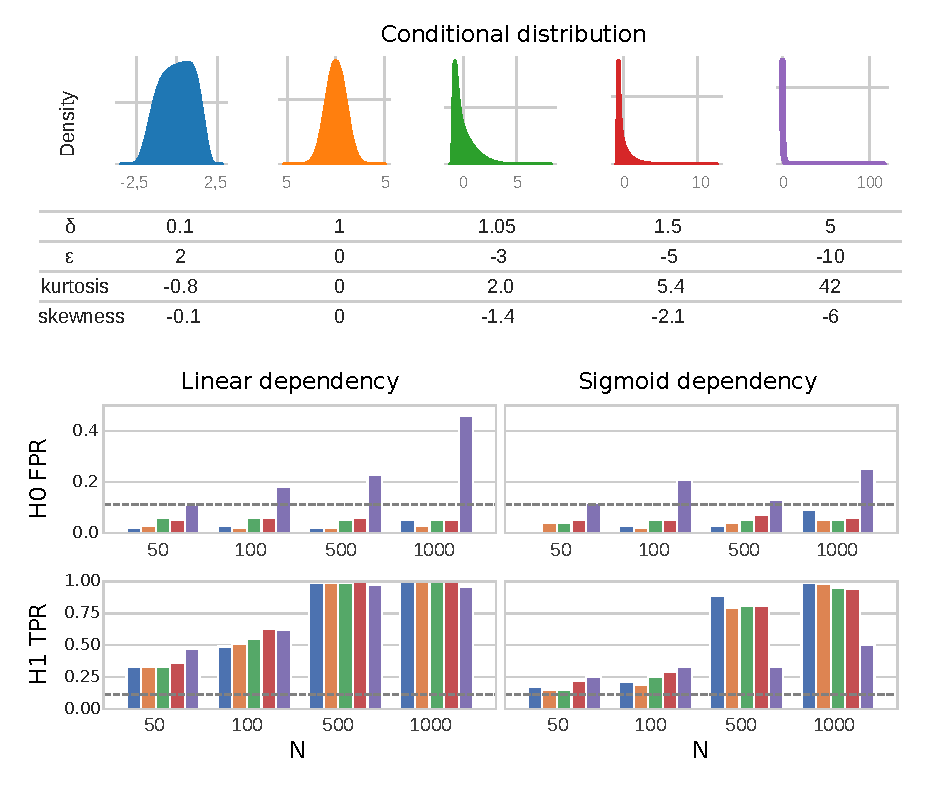
\includegraphics[width=0.40\paperwidth]{fig/sim_non-norm.eps}
  \caption{\textbf{Robustness of conditional permutation based confound testing to the violation of normality assumptions for $\y$ and $\c$.} \\
  Simulations included variables with five different degrees of non-normality (A), as introduced with various $\delta$ and $\epsilon$ values of the \emph{sinh-arcsinh} transformation, from normal (left) to severely skewed and heavy tailed (right). Fisher's kurtosis and skewness is given for each at the bottom of panel A. Panel (B) depicts false positive rates in the simulations under H0, separately for different signal-in-confounder ratios (here identical to $w_{y}$).
  Vertical axis shows type I error rate. The nominal type I error rate of $alpha=0.05$ is shown with a vertical dashed line. Panel (C) shows how violation of the normality assumption affects power. Boxplots show the mean power over simulation cases, grouped by confound-to-target ratio and sample size.}
  \label{fig:sim-non-normal}
\end{figure}

Simulations based on normally distributed data justified that the proposed confounder tests - in line with theory - provide a valid type I error control (For detailed results, see \ref{fig:sim-normal} for the 'partial' test on numerical data and Supplementary Figures \ref{fig:sim-ccc-full}, \ref{fig:sim-ccb-partial}, \ref{fig:sim-ccb-full}, \ref{fig:sim-bbc-partial}, \ref{fig:sim-bbc-full}, \ref{fig:sim-bbb-partial} and \ref{fig:sim-bbc-full} for the partial test on categorical data and the full tests on both numeric and categorical data). 
In case of a valid test, the expected type I error rate in the null hypothesis simulation cases (first row and first column of the figures) is less then or equal to the alpha level (0.05). The upper 95\% confidence limit for the type I error rates for one simulation case (i.e. a single tile on the figures) is 0.11 (binomial confidence intervals with 100 repetitions). 
The results suggest, that the proposed tests are somewhat overly conservative if the model has a high predictive performance (type I error rates closer to 0 than expected).

Simulations with non-normal data showed that the proposed methods are remarkably robust to the violation of normality assumptions for the target variable $\y$ and the confounder $\c$ and, as expected, completely non-parametric regarding the distribution of the predictions $\yhat$). The six simulation cases of normality violation, shown on Figure \ref{fig:sim-non-normal}, involved various \emph{sinh-arcsinh} distributions, form normal (Fisher's kurtosis: 0, skewness) to severely skewed and heavy tailed (kurtosis: 42, skewness: 6).
The results show that the violation of normality - as expected - increases the type I error rate, but the increase - depending on the application - might not be severely problematic up to kurtosis and skewness values as high as 5 and 2 respectively. Furthermore, in terms of type I error rate, normality violation becomes less problematic in case of high predictive performance (high association between the predicted and observed values).

\subsubsection*{Power}

Power estimates for the 'partial' test (with normality) are shown on Figure \ref{fig:sim-normal}. Notably, with sample sizes as large as 1000, a confounder contributing to only 0.4-0.6\% to the variance of the predictions can already be successfully detected ($w_c = 0.05 - 0.07$) with a power of 60-90\%. With a sample size of 500, a confounder contributing to only 1.4-3\% to the variance of the predictions can be detected ($w_c = 0.1 - 0.14$) with a power greater than 80\% in most of the simulation cases. A sample size of 100 yields an approximate power of 60-100\% for a confounder-variance of 6-7\% ($w_c = 0.2 - 0.21$) in most of the cases. Finally, even with a relatively low sample size of 50, the same amount of confounder variance is detected with a power of at least 50\%. If the confounder explains more than 15\% of variance, it is almost certainly detected with $n \geq 50$.

Violation of the normality assumptions for $\y$ and $\c$ has a negative effect on the power of the tests, however the loss of power is low or even negligible, if normality is not extremely violated (first 4 distributions on Fig. \ref{fig:sim-non-normal}A) and the confounder-to-signal ratio is greater or equal then 0.3 (Fig. \ref{fig:sim-non-normal}C).

\subsection{Neuroimaging data}
\subsubsection*{HCP dataset}

\begin{figure}[!b]
  \centering
  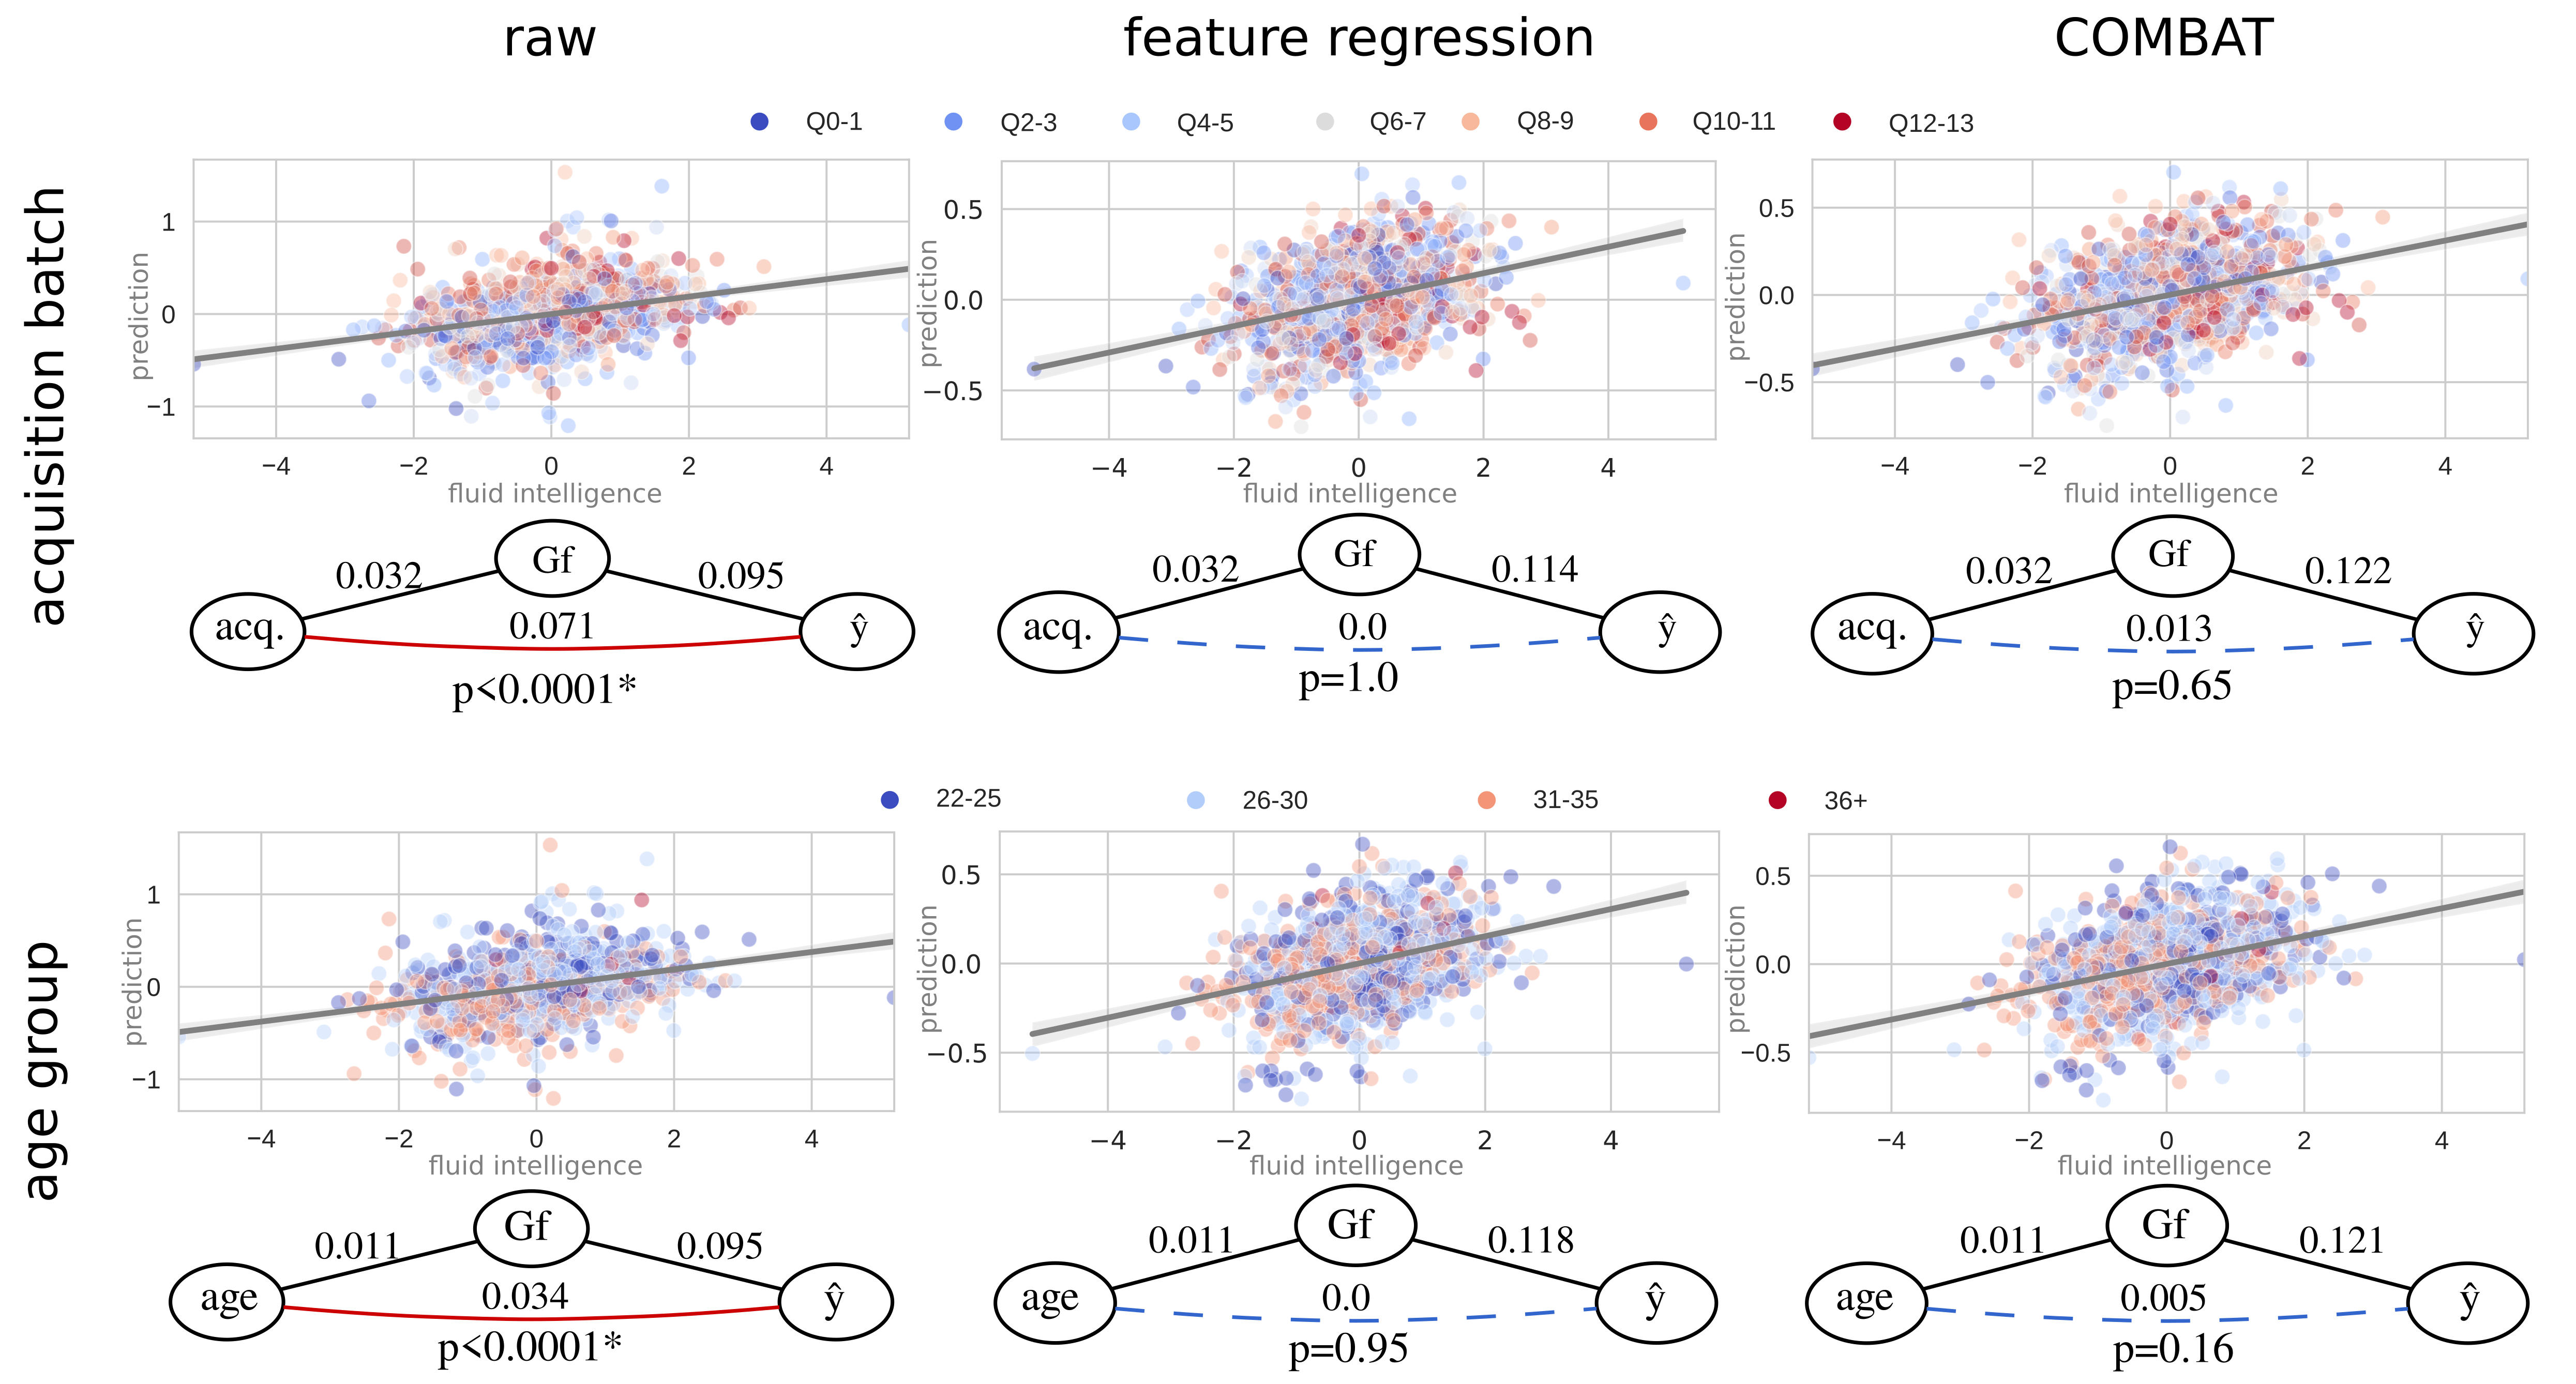
\includegraphics[width=0.75\paperwidth]{fig/fig_hcp.png}
  \caption{\textbf{Acquisition- and age-bias of fluid IQ prediction in the HCP dataset.} \\
  Scatter plots and regression lines (with 95\% confidence intervals) show the association of the observed (horizontals axis) and predicted (vertical axis) fluid intelligence scores with various confound regression strategies. Color-coding of the confounder variables (top: acquisition batch, bottom: age group, as shown by the corresponding legends) reveals confounder-bias for both acquisition and age in the models trained on the raw data. This bias is robustly detected by the proposed 'partial' confounder test ($p<0.0001$) and seems to be effectively mitigated by both feature regression and COMBAT.
  Relation between the observed ($\hat{y}$) and predicted IQ scores and the confounder variables is shown by the graphs as $R^2 values$. Both confound mitigation techniques, but especially COMBAT, improves the predictive performance of the models.
  Solid red line between the confounder and the prediction means significant confounder bias, whereas blue dashed line denotes that confounder testing provided no evidence for bias. P-values are determined with the 'partial confound test'. P-values of the 'full' confound test were all less then 0.0001, i.e. confounder did not fully drive prediction for any of the models.
  }
  \label{fig:hcp}
\end{figure}

Both acquisition batch and age group were statistically significantly associated with fluid intelligence ($R^2=0.032$ and $0.011$ and $p<0.001$ and $=0.001$, respectively, see also Table \ref{tab:unconditional-pvals}). The model trained on the raw (unadjusted) connectivity features predicted fluid intelligence with a medium effect size ($R^2=0.095$, $p<0.001$).
The partial confounder test revealed that the model was significantly biased both by age group and acquisition batch (both $p<0.0001$, first column of Fig. \ref{fig:hcp}) with later phases of the acquisition and lower age being weakly-moderately ($R^2=0.071$ and $0.034$, respectively) associated to larger predicted values.

After applying confound mitigation approaches (feature regression or COMBAT) the partial confound test did not provide evidence of confounder bias anymore ($p > 0.05$ for all, second and third columns of Fig. \ref{fig:hcp}), neither for acquisition batch nor for age. Both feature regression and COMBAT increased the predictive performance in the case of both confounders, with COMBAT providing best performances ($R^2=0.122$ and $0.121$ when applied to remove the effect of acquisition and age, respectively).

The full confounder test was highly significant ($p<0.0001$) for all models, indicating that neither of the models were exclusively driven by the confounds.

\subsubsection*{ABIDE dataset}

\begin{figure}[!b]
  \centering
  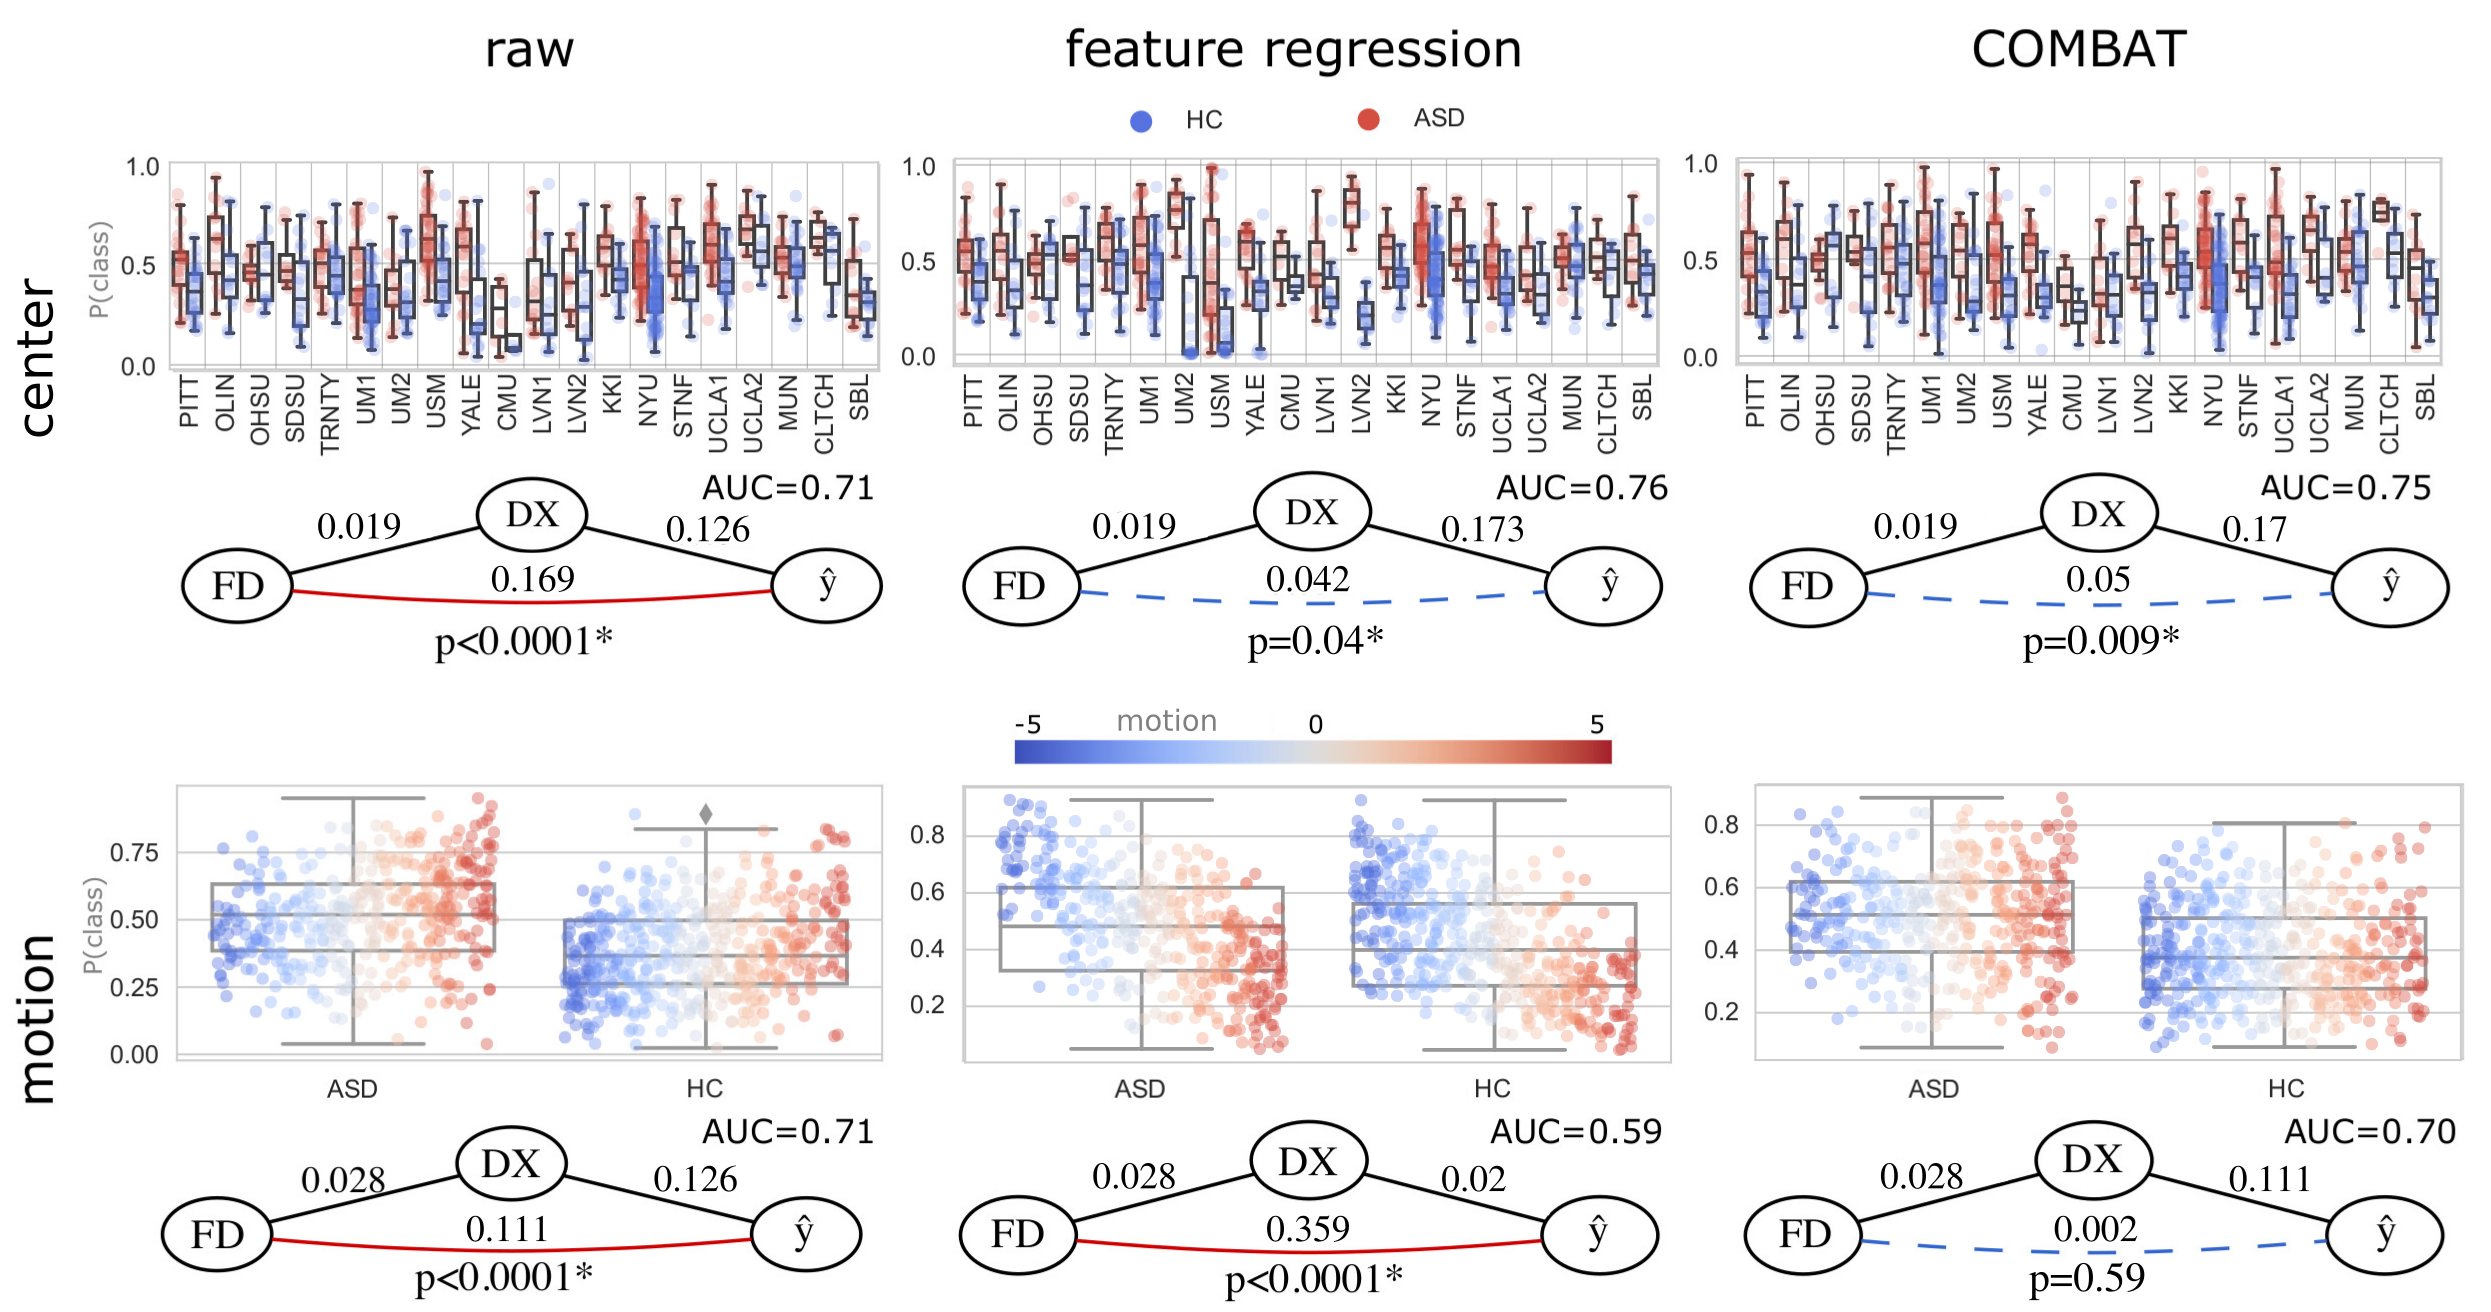
\includegraphics[width=0.75\paperwidth]{fig/fig_abide.png}
  \caption{\textbf{Center- and motion age-bias of ASD diagnosis prediction in the ABIDE dataset.} \\
  Boxplots and points show the predicted class probabilities (0: HC, 1: ASD), separately for the HC and ASD groups. In the top panel, predictions are plotted for each center separately and color indicates the true diagnosis (DX). AT the bottom plot, color indicates the normalized index of in-scanner motion (based on mean framewise displacement, mean FD). The proposed confounder test reveals significant center- and motion-bias in the model trained on the raw data (p<0.0001). While center bias seems to be effectively mitigated by feature regression, the same technique fails to remove motion-bias (actually introduces a paradoxical negative bias). COMBAT seems to effectively remove the effect of both confounders on the predictions and improves the predictive performance of the models in both cases.
  Relation between the observed ($\hat{y}$) and predicted IQ scores and the confounder variables is shown by the graphs as $R^2 values$. Solid red line between the confounder and the prediction means significant confounder bias, whereas blue dashed line denotes that confounder testing provided no evidence for bias. P-values are determined with the 'partial confound test'. P-values of the 'full' confound test were all less then 0.0001, i.e. confounder did not fully drive prediction for any of the models.
  }
  \label{fig:abide}
\end{figure}

Imaging center and in-scanner motion (normalized mean framewise displacement) were statistically significantly associated with ASD diagnosis ($R^2=0.019$ and $0.028$, respectively, $p<0.001$ for both, see also Table \ref{tab:unconditional-pvals}). The model trained on the raw (unadjusted) connectivity features predicted diagnosis with a medium effect size ($R^2=0.126$, $ROC AUC = 0.71$, $p<0.001$).
The partial confounder test revealed that the raw model was significantly biased both for age group and acquisition batch (both $p<0.0001$, see first column on Fig. \ref{fig:abide}). Several sites (e.g. Carnegine Mellon University, University of Leuven, Social Brain Lab UMC Groningen) and lower motion being weakly-moderately ($R^2=0.169$ and $0.111$, respectively) associated to a lower probability for the participant to be assigned to the ASD group by the model.

Both feature regression and COMBAT seemed to significantly attenuate the effect of center, however the partial confound test still provided evidence for a significant center-bias ($p=0.04$ and $0.01$ for feature regression and COMBAT, respectively, see the second and third columns of the first row on Fig \ref{fig:abide}). 

When trying to mitigate the effect of in-scanner motion (bottom row on Fig \ref{fig:abide}), feature regression obviously failed to remove the motion-bias from the model and, in fact, it introduced a paradoxical inverse dependence of the predictions on motion estimates. The partial confounder successfully detected the resulting strong bias ($p<0.0001$). Applying COMBAT to remove the effect of motion (by using binned motion estimates), in turn, seemed to effectively mitigate motion-bias, as suggested by the partial confound test ($p=0.64$, bottom right panel of Fig \ref{fig:abide}).

Both feature regression and COMBAT considerably improved the predictive performance when mitigating center-effects ($R^2=0.111$ and $0.132$ and $AUC=0.76$ and $0.75$, respectively). With both feature regression and COMBAT, however, the effort of mitigating motion effects happened at the cost of a drop in predictive performance ($R^2=0.02$ and $0.111$ and $AUC=0.59$ and $0.70$, respectively)

The full confounder test was highly significant ($p<0.0001$) for all models, except when regressing-out motion from the features ($p=0.09$) Indicating that this model might have been (almost) exclusively driven by motion artifacts.

% tab:unconditional-pvals
\renewcommand{\arraystretch}{1.2}
\begin{table}
\centering
\begin{tabular}{lll|ll|ll|ll|ll} 
dataset & conf. & method & $R^2_{y, c}$ & $p_{y, c}$ & $R^2_{\hat{y}, c}$ & $p_{\hat{y}, c}$ & $R^2_{\hat{y}, y}$ & $p_{\hat{y}, y}$ & partial test & full test  \\
\hline
HCP & acq.  & raw      & 0.032 & <0.001 & 0.071 & <0.001  & 0.095 & <0.001 & \textbf{<0.0001} & <0.0001 \\
    &              & f.reg.    & & & 0.011 & 0.477 & 0.105  & <0.001  & 0.73 & <0.0001 \\
    &              & COMBAT    & & &0.013 & 0.4 & 0.122  & <0.001  & 0.65 & <0.0001\\
\hline
    & age   & raw       & 0.011 & 0.001  & 0.034 & <0.001  & 0.095  & <0.001 & \textbf{<0.0001} & <0.0001 \\
    &       & f.reg.    & & &0.004 & 0.052 & 0.114  & <0.001  & 0.2 & <0.0001 \\
    &       & COMBAT    & & &0.005 & 0.048 & 0.121 & <0.001 & 0.16 & <0.0001 \\
\hline
ABIDE   & center   & raw       & 0.019  & <0.001 &  0.169 & <0.001& 0.126     & <0.001 & \textbf{<0.0001} & <0.0001 \\
        &          & f.reg.    &  & &  0.042 & 0.007 & 0.173     & <0.001 & \textbf{0.04} & <0.0001 \\
        &          & COMBAT    &  & &  0.05 & 0.001 & 0.17     & <0.001 & \textbf{0.009} & <0.0001 \\
\hline
        & motion   & raw       & 0.028 & <0.001 & 0.111    &  <0.001 & 0.126    & <0.001 & \textbf{<0.0001} & <0.0001 \\
        &          & f.reg.    & & & 0.359    & <0.001  & 0.02   & <0.001 & \textbf{<0.0001} & 0.1 \\
        &          & COMBAT    & & &  0.002 & 0.19 & 0.111     & <0.001 & 0.59 & <0.0001 \\
    

\end{tabular}
\caption{\label{tab:unconditional-pvals} Unconditioned coefficients-of-determination, the corresponding p-values and the p-values of the partial and full confounder tests for all investigated models. Significant confoudner bias is denoted by bold font.}
\end{table}

%%%%%%%%%%%%%%%%%%%%%%%%%%%%%%%%%%%%%%%%%%%%%%%%%%%%%%%%%%%%%%%%%%%%%%%%%%%
\section{Discussion}

Confounder-bias can significantly harm the generalizability and biomedical validity of predictive models. Testing confounder-bias of predictive models can be achieved by considering the "confounder-problem" as assessing \emph{conditional independence} between the predicted values and either the target or the confounder variable. These two scenarios result in two different test, testing whether the model is partially or fully driven by the given confounder.
Importantly, in predictive modelling, the model predictions often follow a non-normal distribution, thus any test for confounder bias must be, at least partly, non-parametric.
However, as shown by \citet{shah2020hardness} in their 'no free lunch' theorem, it is effectively impossible to establish a fully non-parametric conditional independence test with a valid type I error control and non-trivial power.
Here I propose the use of the conditional permutation test (CPT) of \cite{berrett2020conditional} to test confounder bias in predictive models. Adapting this approach for the confounder testing problem makes it possible to place assumptions about the joint distribution of only two out of the three variables involved; that is, it allows constructing both the partial and full confounder tests so that no assumption is made about the distribution of the model output. 
The tests are made available in the python package \emph{mlconfound} which builds upon a parallelized, computationally effective implementation of the Markov-chain Monte-Carlo based parallel pairwise sampler of \cite{berrett2020conditional}. It utilizes coefficient of determination ($R^2$ or pseudo $R^2$ in case of categorical confounder or classification) as a test statistic and assumes that the conditional distribution between the target variable and the confounder is normal. The partial and full confounder tests available in \emph{mlconfound} can be uniformly applied for any predictive model, given that realistic (e.g. cross-validated) model predictions can be obtained. Both tests require only the target variable, the model predictions and the putative confounder as input, thus, they can be performed with a negligible extra computational cost; re-fitting the model is not required.

As expected from theoretical justification, both tests displayed a valid type I error control in the simulations with the necessary assumptions, that is, even if $\yhat$ is not normally distributed. In fact, the tests were found to become somewhat conservative (i.e. lower than expected type I error rates ) in the case of high-performance predictive models (when the $R^2$ between the predicted and observed values is greater than 0.7). 

Even tough the tests valid type I error control is justified by theory and reinforced by the simulations, a low statistical power could significantly limit their usefulness. The simulations presented in this paper revealed that both tests have a high, practically relevant power in a wide variety of scenarios; with different strength of the association between the target and the confounder, varying predictive performance, various sample sizes and different true confound-to-signal ratios in the predictions. Considering the partial test, if we apply \citeauthor{cohen2013statistical}'s terminology for the effect size of the confounder bias, sample sizes around 500-1000 can robustly identify a very weak confounder bias (e.g a confounder explaining 1-2\% of the variance in the prediction). A lower sample size of 100 will still very likely identify medium sized confounder-biases (around 9\%). Strong biases  (>25\%) can be very robustly detected with sample sizes as low as 50. 
As expected, the power of the full confounder test is very similar to the partial test, since the only difference is that the conditional contribution of the target to the prediction is investigated, instead that of the confounder.

While different biomedical applications might consider different amounts of bias to be relevant, an a-priory power calculation can help identifying the necessary sample size in order to exclude the possibility of a relevant confounder bias with a high probability.

Next to statistical power, the practical applicability of the proposed tests is also highly affected by their robustness to violations of the normality assumptions on the conditional distribution of $\y$ and $\c$. Importantly, the simulations strongly suggest that both tests are strikingly robust to the violation of this assumption. Type I error is well controlled even in case of highly skewed and heavy tailed distributions (kurtosis > 5, skewness > 2) and gets significantly inflated only with extreme violations of normality (see the purple distribution on Fig. \ref{fig:sim-non-normal}). Due to the conservatives of the tests, if the predictive model is very accurate, even this extremely skewed and heavy tailed distribution resulted in lower than the nominal type I error rates.

Non-normality has a negative effect on the power of both tests, however, the decrease in power is in most cases small or even negligible and gets only more pronounced if the sample size and/or the confounder-effect is low.

Validity, power and robustness renders the proposed tests as unprecedented tools for model diagnostics in a wide spectrum of predictive modelling scenarios.
For instance, in biomedical research, confounder-bias has previously often been investigated (if investigated at all) by testing the (unconditioned) association between the confounder variable and the predictive values, see e.g. \citep{spisak2020pain}. However, the significance of the unconditioned association does not necessarily imply a significant confound-bias of the model, especially if the confounder is also associated to the true target variable. In this case, namely, the model still might not be directly driven by the confounder and the dependence of the predictions on the confounder might be only marginal, to be explained solely by the confounder-target association. 
Two examples for this situation can be found in the presented analysis of real data; when applying COMBAT to mitigate age-bias in the HCP data and when regressing out the center-effect from the ABIDE data (see Table \ref{tab:unconditional-pvals}).

Arguably, in certain applications, the researcher might aim to fully eliminate confounder-related variance of the predictions and, in this case, testing unconditional independence between the confounder and the predictions might be sufficient. However, a much more realistic aim is to construct models that allow a reasonable degree of marginal confounder-association of the predictions, but are likely not directly driven by confounder-information, i.e. the prediction-confounder association is proportional to, and can likely be fully explained by, the target-confounder association.
Put simply, this is what is tested by the proposed partial confounder test.

Obviously, a true confounder bias might still be present in the model, even if the the target-confounder association likely explains the prediction-confounder association, i.e. the model might still use the confounder's effect on the features (e.g artifacts) to construct the corresponding part of the variance in the prediction. Nevertheless, in most of the cases, it does not seem likely that the model, at the same time, (i) misses that specific "part" of the target variable's variance in the features that is shared with the confounder (ii) captures exclusively that component of the confounder's variance in the features that is needed to mimic an unbiased model.
Usually a much more plausible explanation is that a direct confounder effect in the model output is simply negligible (e.g because it is not to be found in the features after confound mitigation).

Among the many potential areas of applications, the proposed tests could be certainly useful in translational neuroscience. A characteristic example is provided by the novel field of "predictive neuroscience", where applying predictive modelling and machine learning on functional neuroimaging data holds a great potential for both revolutionizing our understanding of the physical basis of mind and delivering clinically useful tools \citep{woo2017building, wager2013fmri, spisak2020pain}. However, the presence of confounders typical for biomedical research (e.g. sample demographics, center-effects) and specific to the data acquisition and processing approach (e.g. imaging artifacts) presents a great challenge to these efforts and is, currently, often largely neglected.

To demonstrate the usefulness of the proposed tests in detecting various types of confounder-bias, here they have been deployed in two research settings (a regression and a classification problem) where specific types of confounding effects have previously been described. 
First, functional connectivity data from the Human Connectome Project (HCP) \citep{van2013wu} was used to build predictive models of fluid intelligence and to test for the previously discussed confounding effect of age \citep{lohmann2021predicting, dubois2018distributed} and,  additionally, the - somewhat underdiscussed - batch-like effect of acquisition date of the data within the course of the data acquisition process.
Second, functional connectivity data from the ABIDE \citep{di2014autism} database was used to investigate the potential motion- and center-bias (as previously reported by e.g. \cite{spisak2014voxel, spisak2019optimal, gotts2013perils}) when training models that aim to predict ASD diagnosis.

The hypothesised confounder effects were clearly present in both datasets.

In case of the HCP dataset, the weak but statistically significant association between age and IQ predictions could likely exaggerate to a serious bias when testing the model on data of participants outside of the (relatively narrow)
age range of the HCP sample. In this case, the bias would likely significantly harm the out-of-sample generalizability of this model. The bias of the same model to 'acquisition batch' (phase of the study the acquisition belongs to) can also be problematic and it has not yet been thoroughly discussed in case of the HCP dataset. There can be manifold reasons for the observed association. Fluid intelligence of the participants might be, for instance, affected by a changing selection bias during participant recruitment (e.g. as a consequence of the human connectome project receiving an increasing degree of public interest during its course, the sociodemographic and educational characteristics of the volunteer sample might have changed over time). To explain the associated change in the target variable, the model might utilise changing characteristics of the imaging data (caused by e.g. slight changes in the calibration settings of the measuring equipment or the changing level of experience of the research staff). This is obviously undesirable for any brain-based predictive model of fluid intelligence.

In the ABIDE dataset, neither the medium-strong center-bias nor the age-bias is surprising but both are obviously problematic for a diagnostic model of ASD. For instance the model trained on the raw (unadjusted) features - depending on the calibration of the predicted class probabilities - might classify all participants form e.g. the CMU (Carnegie Mellon University) center as neurotypical control participants. It's easy to see that this bias can possibly lead to a very low predictive performance on out-of-center data. Similarly, a model biased by motion - next to having questionable neuroscientific validity - might systematically fail in populations with higher motion or altered motor characteristics (as known e.g. for ADHD \citep{eloyan2012automated}).

Confounder mitigation techniques, with one exception, tended to decrease confounder bias. The partial confounder test provided detailed insights into the effectiveness of the techniques for each confounder. In the HCP data, it revealed that both the acquisition-bias and the age-bias was very effectively removed by both feature regression and COMBAT (p>0.05 for all). Given the high power of the test at the sample sizes of the HCP dataset ($N=999$), any remaining confounder-bias is most probably very safely negligible and well out of the range of practical relevance.

On the other hand, the partial confoudner test also showed, that the performance of the investigated confound mitigation techniques is much less convincing for the ABIDE dataset. The center-bias of the classification in this massively multi-center dataset was, namely, found to be significant, even after feature regression and COMBAT. Nevertheless, the p-values returned by the partial confounder test were larger with two orders of magnitude than without any confound mitigation, suggesting that a large part of the center effects was still successfully removed by both approaches. While determining the relevance of the remaining bias is to be performed based on the experimental context and the requirements towards the predictive marker, significant p-values of the partial confounder test generally suggest that these models would either require more effective data harmonization or a validation on external data, that confirms the low practical relevance of the amount of bias.

Motion-bias in the ABIDE dataset was not detectable anymore after COMBAT, but remained highly significant after feature regression.
Interestingly, in the latter case, the association between the confounder and the predictions become even stronger than before but with an opposite sign. Meanwhile, the prediction performance substantially dropped (although still remained statistically significant). 
A possible explanation to these phenomena is that in-scanner motion, as previously described \citep{fournier2010motor, anzulewicz2016toward}, has manifold links to ASD and, therefore, regressing out motion estimates from the connectivity features might eliminate a significant amount of signal-of-interest (especially in functional connections that are themselves directly associated with motor deficits in ASD).
On the other hand, motion artefacts were previously shown to display complex spatiotemporal patterns in fMRI-based functional connectivity estimates \citep{spisak2014voxel} and simply regressing them out of the features is far from being sufficient for removing their effect on the model. The so-called "residual motion artefacts" and their regional interactions, as described in the referenced work, might be responsible for the paradox behavior of this model, which raises caution for using feature regression to mitigate the effect of motion artifacts and similarly complex confounders.
 
 As COMBAT was originally developed for harmonizing effects of categorical variables (e.g. center or batch), using it to remove the effect of continuous variables is not trivial. The presented method of inputting the binned "motion groups" into COMBAT resulted in an efficient removal of motion-bias and, at the same time, preserved a significant amount of signal-of-interest. 
 Nevertheless, inputting discretized versions of continuous variables into COMBAT might be sub-optimal and raises further questions e.g regarding the optimal number of bins used during the discretization.
 
 In sum, the application of the partial confounder test suggests that confounder-bias should be much more carefully investigated and reported in studies utilizing predictive modelling and machine learning as (i) variables as trivial as the date of the acquisition can cause significant model-bias and (ii) in certain situations, a sufficient mitigation of confounder-bias requires more effective solutions than feature regression and COMBAT. The partial confounder test can be considered as a useful objective benchmark to guide the search for a suitable confounder mitigation approach.
 
While the real data examples in this paper were not typical cases of the potential applications of the full confounder test, it has still provided important insights into model biases. Namely, in the case of the aforementioned paradox motion-regression model in the ABIDE dataset, the full confounder test did not provide any evidence that the model captures any extra variance over that explained by the confounder. In other words, the test accepted the null hypothesis of full model bias, suggesting that this model might be, in fact, almost exclusively driven by motion artifacts.
For all other models, the full confounder test confirmed that - even if there was a significant confounder-bias - the model was not fully driven by the confounder (in other words, the target and the prediction were not independent, given the confounders).
This examples highlights that the full confounder test might become useful in exploratory phases of model development, where models might be still severely biased and the questions is whether there is any biomedical relevant signal captured by the model, at all.


%%%%%%%%%%%%%%%%%%%%%%%%%%%%%%%%%%%%%%%%%%%%%%%%%%%%%%%%%%%%%%%%%%%%%%%%%%%
\section{Conclusion}

The lack of rigorous statistical tests for confounder-bias significantly hampers the development of predictive models in many fields of research. Even tough several approaches for mitigating the effects of counfounder variables in machine learning have been recently proposed, these can potentially remove signal-of-interest together with the confounder signal and an informed decision about confound mitigation strategy is impossible without a proper test of confounder-bias.

To fill this critical gap in predictive model development, here I proposed two novel tests, the partial and the full confounder tests, which probe the null hypotheses of 'no confounder-bias' and 'full confounder-bias', respectively. Both approaches are based on a recently published framework for conditional permutation testing, with a mathematical justification of valid type I error control. The tests were constructed so that they do not place any assumption on the distribution of the model predictions and require only the target variable, the model predictions and the putative confounder as input, that is, they can be performed with a minimal computational overhead; without needing to re-fit the model.

Given their simplicity, high statistical power, robustness to the violation of the assumptions and thanks to the computationally effective implementation (available in python package \emph{mlconfound}\footnote{\href{https://mlconfound.readthedocs.io}{https://mlconfound.readthedocs.io}}), the tests are deployable in a wide variety of applications.

As demonstrated on functional brain connectivity-based predictive models of fluid intelligence and autism, the tests can guide the optimization of the confound mitigation strategy and allows quantitative, statistical assessment of the robustness, generalizability and neurobiological validity of predictive models in biomedical research, thereby paving the way for the development of clinically useful machine learning biomarkers.

\bibliographystyle{apalike}  
\bibliography{references}

\newpage
\section{Supplementary Material}
\beginsupplement

\begin{figure}[H]
  \centering
  \fbox{
   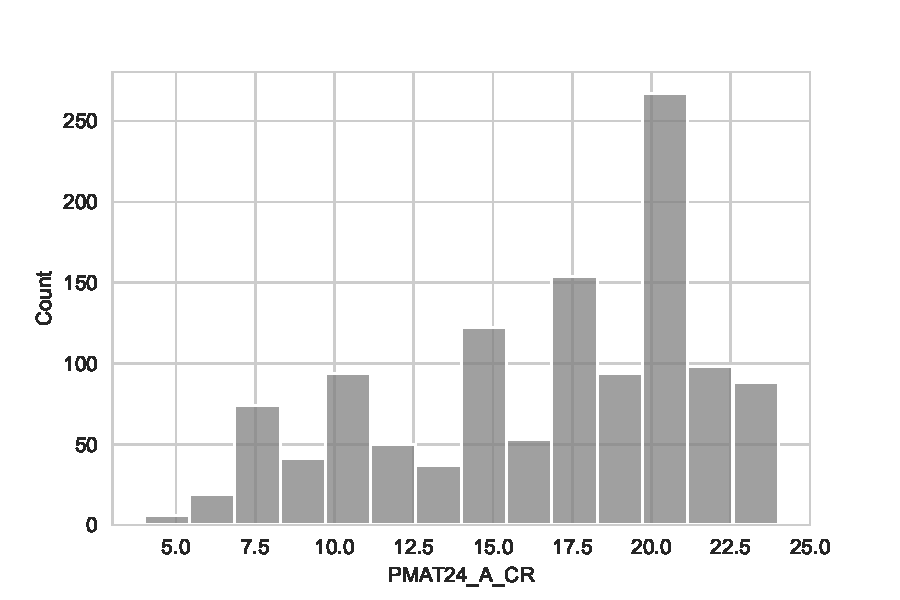
\includegraphics[width=0.36\paperwidth]{fig/hcp_iq_nonnorm_hist.pdf}
   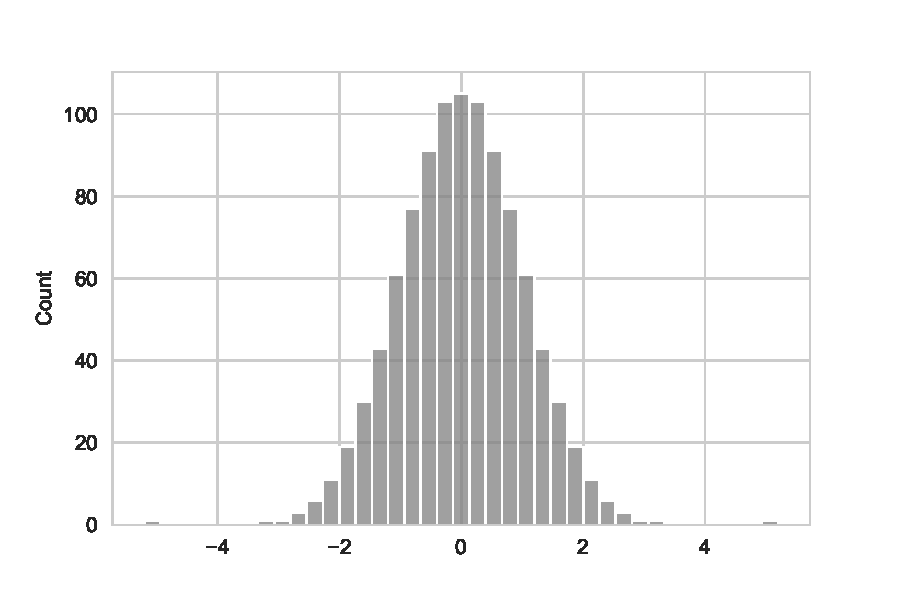
\includegraphics[width=0.36\paperwidth]{fig/hcp_iq_quanttrf_hist.pdf}
   }
  \caption{Histogram of fluid intelligence score in the HPC dataset, before (left) and after (right) quantile transformation.}
  \label{fig:hcp-hist}
\end{figure}

\begin{figure}[H]
  \centering
  \fbox{
   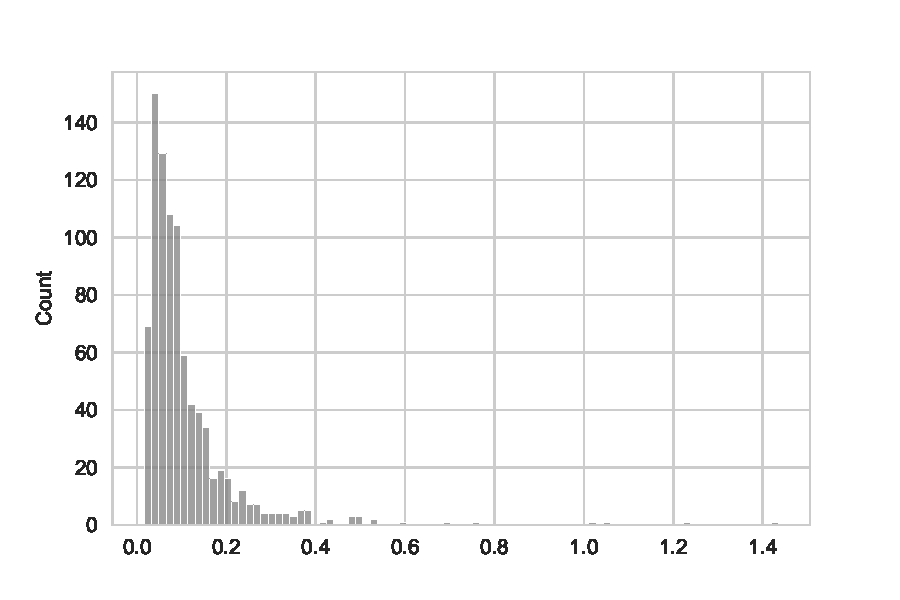
\includegraphics[width=0.36\paperwidth]{fig/abide_motion_hist.pdf}
   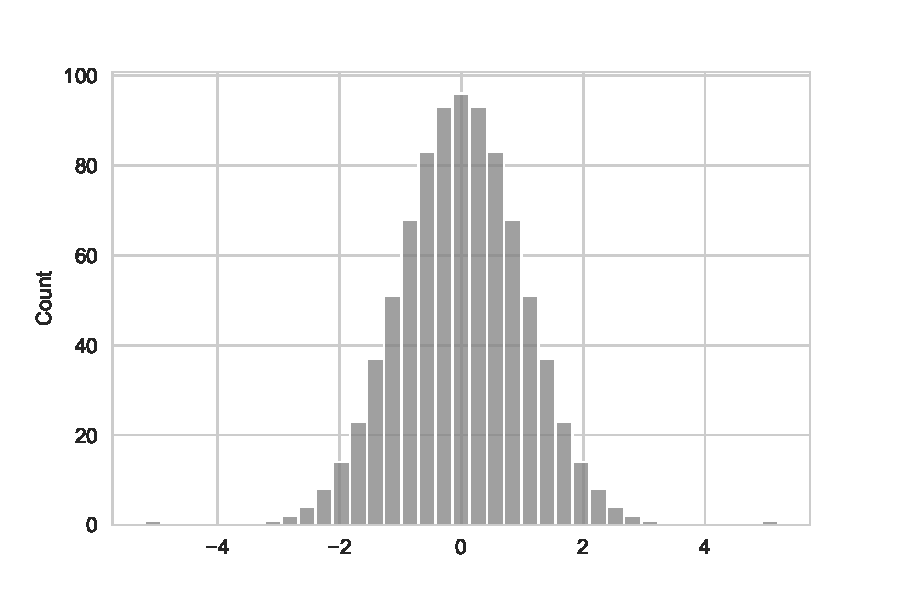
\includegraphics[width=0.36\paperwidth]{fig/abide_motion_quanttrf_hist.pdf}
   }
  \caption{Histogram of mean framewise displacement in the ABIDE dataset, before (left) and after (right) quantile transformation.}
  \label{fig:abide-hist}
\end{figure}


\end{document}
